\chapter{Implementation}

In this chapter, we first give a high level overview of the possibilities for parallelization and data reuse in the implementation of definition-based cross-correlation algorithm, introduced in section \ref{sec:cross_corr_def}. We then describe a basic implementation of the definition-based algorithm with all its problems. Next, we try to mitigate the problems of the basic implementation by introducing a simple implementation based on Warp Shuffle instructions. We continue with several optimizations and create a family of implementations based on Warp Shuffle instructions. Lastly we implement a second family of optimizations designed to solve problems with low occupancy, based on assigning the computation of a single job to larger group of threads.


The definition-based algorithm has several properties which allow for parallelization, optimization through data reuse and distribution of work. Figure \ref{fig:cross_corr_shifts} depicts the output matrix with corresponding relative shift of the two input matrices, which defines the computed overlap. As described in Section \ref{sec:cross_corr_opt}, each element of the output matrix can be computed independently in parallel.

\begin{figure}[ht]
	\fontsize{6}{8}\selectfont
	\centering
	\def\svgwidth{0.55\textwidth}
	% Must be relative to current directory
	% as input ignores graphicspath, which is
	% only for includegraphics{}
	\input{./img/overlap-Shifts.pdf_tex}
	\caption{Result matrix with corresponding relative shifts.}
	\label{fig:cross_corr_shifts}
\end{figure}

Each overlap defines a unique set of element pairs which are to be multiplied. Each of these pairs of overlapping elements belongs to exactly one overlap of the two matrices.


\section{Parallelization}
\label{sec:implementation_parallelism}
In this section, we first highlight the independent parallel tasks present in the definition-based cross-correlation algorithm.  

% REFERENCE file:///home/karel/skola/diplomka/crosscorr/papers/related_work/IJIGSP-V5-N12-4.pdf distributes different shifts of 1D cross correlation between different PCs in LAN. We go step further and distribute each shift to separate treads

The partitioning of the problem into tasks is inspired by \citet{paper:cross_corr_tasks}, who distributes computation of a one dimensional cross-correlation of two signals between nodes in a local network. The range of possible delays between the two signals is split between nodes. In this thesis, we talk about shifts instead of delays as we are computing different ways two matrices overlap. We go further and instead of assigning ranges of shifts, we partition the problem into single shifts or even further, assigning part of a shift computation as a job.

% REFERENCE file:///home/karel/skola/diplomka/crosscorr/papers/related_work/Honz%C3%A1tko-Kruli%C5%A12019_Article_AcceleratingBlock-matchingAnd3.pdf each thread processes patches which mostly overlap, similar to our implementation

The partitioning is also similar to the problem studied by \citet{paper:krulis_3d_block}, as the problem of 2D cross-correlation is very close to the problem of block-matching in the type of independent parallel tasks it can be partitioned into. Block-matching takes a submatrix, called reference patch, and goes through all submatrices (patches) of the same size in a neighborhood around the reference patch, computing the distance between them and the reference patch using some distance function and giving as output patches with distance lower than some threshold. As described by \citet{paper:krulis_3d_block}: "The block-matching algorithm offers many opportunities
for employing data parallelism. Multiple reference patches
can be processed concurrently, distances between reference
patch and patches in its neighborhood (the $n \times n$ window)
can be computed concurrently, and even the L2 distance
function itself can be parallelized internally."

Definition-based computation of 2D cross-correlation provides similar possibilities for parallelization, where multiple pairs of input matrices can be processed concurrently, each possible overlap of two input matrices can be computed concurrently and even each pair of overlapping items in given overlap can be processed independently and in parallel. 

\subsection{Two matrices}
When we focus on the computation of cross-correlation between two matrices, called \textit{one-to-one} in the rest of the thesis, we can reformulate the definition-based algorithm as a problem with two levels of independent parallel tasks, as shown in Figure \ref{fig:cross_corr_one_to_one_tasks}. The top level represents the single output matrix, which with only two input matrices represents the result of the whole computation. The second level of tasks, represented by orange boxes, contains one box for each relative shift of the two input matrices, or in other words each orange box corresponding to a single element of the output matrix. Each shift defines an overlap of the two input matrices, which in turn defines a set of independent subtasks, each subtask representing an overlapping pair of elements of the two input matrices. In Figure \ref{fig:cross_corr_one_to_one_tasks}, the subtasks representing pairs of overlapping elements are represented by yellow boxes. Every such subtask belongs to exactly one second level task, creating a tree structure. The set of subtasks which are children of the same orange box defines a submatrix in both input matrices, as shown in Figure \ref{fig:cross_corr_shifts}.


When we look at the operations, every yellow box represents a single multiplication and every orange box represents a sum of the results of all of its children. 

\begin{figure}[ht]
	\fontsize{5}{6}\selectfont
	\centering
	\def\svgwidth{0.6\textwidth}
	% Must be relative to current directory
	% as input ignores graphicspath, which is
	% only for includegraphics{}
	\input{./img/overlap-Tasks.pdf_tex}
	\caption{Tasks hierarchy in definition-based one-to-one cross-correlation.}
	\label{fig:cross_corr_one_to_one_tasks}
\end{figure}

The goal is to distribute the tasks between workers in such a way that we maximize parallelism, maximize data reuse and minimize the need for communication and synchronization between workers.

\subsection{Many matrices}

With more than two matrices, we add additional tasks to the top level of the task hierarchy shown in Figure \ref{fig:cross_corr_one_to_one_tasks}, creating a forest of trees. As described in Section \ref{sec:cross_corr_forms}, there are several forms of cross-correlation between multiple matrices. For us, the most important of these are:
\begin{enumerate}
	\item \textit{one-to-many} (Figure \ref{fig:implementation_one_to_many}, for example comparing deformation changes in images taken over time),
	\item \textit{n-to-mn} (Figure \ref{fig:implementation_n_to_mn}, for example comparing deformations in time of multiple parts of a single large object),
	\item \textit{n-to-m} (Figure \ref{fig:implementation_n_to_m}, also called \textit{all-to-all}).
\end{enumerate}

\begin{figure}
	\centering	
	\begin{subfigure}{0.4\textwidth}
		\centering
		\def\svgwidth{0.5\textwidth}
		% Must be relative to current directory
		% as input ignores graphicspath, which is
		% only for includegraphics{}
		\input{./img/overlap-OneToOne.pdf_tex}
		\caption{One to one.}
		\label{fig:implementation_one_to_one}
	\end{subfigure}
	\hfill
	\begin{subfigure}{0.4\textwidth}
		\centering
		\def\svgwidth{0.5\textwidth}
		% Must be relative to current directory
		% as input ignores graphicspath, which is
		% only for includegraphics{}
		\input{./img/overlap-OneToMany.pdf_tex}
		\caption{One to many.}
		\label{fig:implementation_one_to_many}
	\end{subfigure}
	\hfill
	\begin{subfigure}{0.4\textwidth}
		\centering
		\def\svgwidth{0.7\textwidth}
		% Must be relative to current directory
		% as input ignores graphicspath, which is
		% only for includegraphics{}
		\input{./img/overlap-NtoMN.pdf_tex}
		\caption{N to MN.}
		\label{fig:implementation_n_to_mn}
	\end{subfigure}
	\hfill
	\begin{subfigure}{0.4\textwidth}
		\centering
		\def\svgwidth{0.7\textwidth}
		% Must be relative to current directory
		% as input ignores graphicspath, which is
		% only for includegraphics{}
		\input{./img/overlap-NToM.pdf_tex}
		\caption{N to M.}
		\label{fig:implementation_n_to_m}
	\end{subfigure}
	
	\caption{Forms of cross-correlation.}
	\label{fig:implementation_forms}
\end{figure}

The \textit{one-to-many} type together with the \textit{one-to-one} type, shown in Figures \ref{fig:implementation_one_to_many} and \ref{fig:implementation_one_to_one} respectively, are subtypes of the \textit{n-to-mn} type and \textit{n-to-m}, as implementations of both of these general types can be used to compute the two simpler types. We separate the \textit{one-to-one} and \textit{one-to-many} types as they offer a greater possibility for caching the single left input matrix.

All of the described types can be partitioned into many \textit{one-to-one} cross-correlations, as shown in Figure \ref{fig:cross_corr_many_tasks}. For both \textit{n-to-mn} and \textit{n-to-m} types, the number of green top level tasks, corresponding to the number of result matrices, is equal to $n*m$. To reiterate, the difference between the \textit{n-to-mn} and \textit{n-to-m} types is that in the \textit{n-to-mn} type, each of the \textit{n} left input matrices is cross-correlated with a different set of \textit{m} right input matrices, whereas in the \textit{n-to-m} type, all \textit{n} left input matrices are cross-correlated with the same \textit{m} right input matrices. Based on this, the \textit{n-to-m} type allows for greater data reuse, as each right input matrix is used multiple times compared to being used just once in the \textit{n-to-mn} type. 

\begin{figure}[ht]
	\centering
	\def\svgwidth{0.8\textwidth}
	% Must be relative to current directory
	% as input ignores graphicspath, which is
	% only for includegraphics{}
	\input{./img/overlap-ManyTasks.pdf_tex}
	\caption{Task hierarchy of types with many matrices.}
	\label{fig:cross_corr_many_tasks}
\end{figure}

As in the case of \textit{one-to-one} type, the meaning of the boxes is as follows:

\begin{itemize}
	\item Each green box represents a pair of input matrices, or equivalently a single output matrix;
	\item Each orange box represents an element in the output matrix, or equivalently a relative shift of the two input matrices;
	\item Each yellow box represents a pair of overlapping elements from the two input matrices.
\end{itemize}

All boxes on a given level can be processed completely independently.  Results of the orange boxes have to be written into the output matrix represented by their green box parent. Each orange box represents a different element of the parent matrix, which allows the writes corresponding to different orange box tasks to be executed without any collisions. All results of the yellow box children of an orange box have to be added together, corresponding to a reduce operation.

% Segway to data reuse and workers

As the number of tasks cannot be reduced, the only directions for optimization are parallelization and data reuse. Even through tasks can be processed independently and in parallel, many tasks can share and reuse data from other tasks. For example, orange boxes from different subtrees representing the same shift between input matrices and sharing the same left input matrix can be computed by reusing the data from the left matrix. Relationships such as this can be used to group tasks into \textbf{jobs} for workers to reuse data or pass data to other neighboring workers to reduce the required memory throughput and keep data closer to the execution units. 

\section{Data reuse}
\label{sec:data_reuse}
To fully utilize the GPU hardware, we cannot rely on parallelization alone, but must keep the data as close as possible to the execution units for fast access. To achieve this goal, we have to group tasks defined in Section \ref{sec:implementation_parallelism} into cooperating groups, mostly for sharing input data. We call these groups \textbf{jobs}.


The two basic levels on which tasks are grouped into jobs in our implementations are:
\begin{itemize}
	\item overlap, grouping one or more orange boxes (output matrix elements) into a single job;
	\item row group or column group, grouping the yellow boxes from a single overlap by rows or columns into jobs.
\end{itemize}

The following subsections describe groupings based on each of these units.

% REFERENCE file:///home/karel/skola/diplomka/crosscorr/papers/related_work/levenstein.pdf with their stripes
This grouping is inspired by \citet{paper:levenstein}, who implement the computation of Levenshtein edit distance on many parallel accelerators, including a GPU. They also solve a slightly different problem in terms of data reuse, as they share intermediate results between threads, whereas we try to reduce the overhead of fetching input data from device memory by passing them between threads to reduce the impact of low arithmetic intensity of each task described in Section \ref{sec:implementation_parallelism}, but the principles employed by \citet{paper:levenstein} can be utilized for both.





\subsection{Overlap}
\label{sec:data_reuse_overlap}

When tasks are grouped on the level of overlaps, i.e. orange boxes in the task hierarchy in Figure \ref{fig:cross_corr_many_tasks}, into jobs, we call that the \textit{overlap} basic job size. With this job size, each job computes one or more elements of the output matrix. The job contains all tasks in the subtree with the assigned orange box as its root, or in all subtrees of all assigned orange boxes if multiple overlaps are grouped into a single job.

Multiple overlaps can be grouped into a single job in several ways. First is the \textbf{multimat overlap} job size, where multiple overlaps (orange boxes) from different output matrices (green boxes) are grouped into a single job. To enable data reuse, overlaps representing the same shift between different matrices are grouped, as shown in Figure \ref{fig:job_size_modifiers}. There are two versions of this optimization:
\begin{itemize}
	\item multimat-right, designed for \textit{n-to-mn} computation type, where job contains overlaps with the same shift between single left input matrix and multiple right input matrices, shown in Figure \ref{fig:job_size_modifiers_n_to_mn};
	\item multimat-both, designed for \textit{n-to-m} computation type, where job contains overlaps with the same shift between multiple left input matrices and multiple right matrices, shown in Figure \ref{fig:job_size_modifiers_n_to_m}.
\end{itemize}

Another way to reuse data is to compute multiple overlaps which are close to each other in a single output matrix. 
We call this the \textbf{multirow overlap} job size. Their proximity in the output matrix corresponds to the shifts of the input matrices being very similar, which in turn means that most of the input data is shared between the overlaps, as shown in Figure \ref{fig:multirow_shared_input}. This grouping is also shown in Figure \ref{fig:job_size_modifiers}. Our implementation groups overlaps from multiple consecutive rows of a single column of the output matrix into a single job. The reasons for this grouping choice are further expanded in Section \ref{sec:multirow_right}.
% TODO: Maybe multirow-right and multirow-both

The \textit{multimat} and \textit{multirow} optimizations can be combined as shown in Figure \ref{fig:job_size_modifiers}.



\begin{figure}[ht]
	\centering	
	\begin{subfigure}{0.4\textwidth}
		\centering
		\def\svgwidth{\textwidth}
		\fontsize{8}{10}\selectfont
		% Must be relative to current directory
		% as input ignores graphicspath, which is
		% only for includegraphics{}
		\input{./img/overlap-JobSizeOverlapSimple.pdf_tex}
		\caption{Grouping in \textit{n-to-mn} type.}
		\label{fig:job_size_modifiers_n_to_mn}
	\end{subfigure}
	\hfill
	\begin{subfigure}{0.4\textwidth}
		\centering
		\def\svgwidth{\textwidth}
		\fontsize{8}{10}\selectfont
		% Must be relative to current directory
		% as input ignores graphicspath, which is
		% only for includegraphics{}
		\input{./img/overlap-JobSizeBoth.pdf_tex}
		\caption{Grouping in \textit{n-to-m} type.}
		\label{fig:job_size_modifiers_n_to_m}
	\end{subfigure}
	
	\caption{Grouping of overlaps into jobs.}
	\label{fig:job_size_modifiers}
\end{figure}

\begin{figure}[ht]
	\centering
	\def\svgwidth{0.5\textwidth}
	\fontsize{8}{10}\selectfont
	% Must be relative to current directory
	% as input ignores graphicspath, which is
	% only for includegraphics{}
	\input{./img/overlap-DataSharedByOverlaps.pdf_tex}
	\caption{Input data shared between neighboring overlaps.}
	\label{fig:multirow_shared_input}
\end{figure}

\subsection{Row group and column group}
\label{sec:data_reuse_row_column_group}

% With work distribution, jobs created from the same overlap do not share any input data, but share data with the jobs with the same ID from neighboring overlaps

With overlaps as the tasks grouped into jobs, load balancing becomes a problem. The amount of work required by each job may differ massively, as illustrated by the two tasks shown by the two overlaps in Figure \ref{fig:row_subset_tasks}. This leads to problems with occupancy once jobs with small amount of work are finished. 

We implement an alternative where instead of grouping overlaps into jobs, we go one step lower in the task hierarchy and group the individual tasks representing multiplication of one overlapping pair of input elements (yellow box) into jobs. This change results in the computation of a single overlap being split into several smaller jobs, improving load balancing between jobs while also increasing parallelism. One problem of this change is the required final reduce operation to consolidate the results of all jobs computing parts of the same overlap.

To enable additional optimizations described in the following sections of this chapter, we choose to group the yellow box tasks into jobs by whole rows of the overlap. The number of rows grouped into a single job is configurable through algorithm argument. This grouping is illustrated in Figure \ref{fig:row_subset_tasks}, where \textit{Max job rows} is the argument of the algorithm. Each overlap with $r$ overlapping rows of the two input matrices is split into $\lceil \frac{r}{max\_job\_rows} \rceil$ jobs, with each job containing at most \textit{max\_job\_rows} consecutive rows. With this distribution, each job represents a submatrix of the overlap with the same number of columns as the original overlap. This also means that all overlaps with the same number of rows will be split into the same number of jobs.

For data reuse, one important observation is that jobs from the same overlap do not share any input data, but jobs with the same ID from neighboring overlaps in the same row of the output matrix(i.e. with the same number of rows in the overlap) will share most of the input data, as shown in Figure \ref{fig:row_subset_data_reuse}.

\begin{figure}[ht]
	\centering
	\def\svgwidth{0.6\textwidth}
	\fontsize{8}{10}\selectfont
	% Must be relative to current directory
	% as input ignores graphicspath, which is
	% only for includegraphics{}
	\input{./img/overlap-JobSizeRowSubset.pdf_tex}
	\caption{Grouping of rows of tasks into jobs.}
	\label{fig:row_subset_tasks}
\end{figure}

\begin{figure}[ht]
	\centering
	\def\svgwidth{0.5\textwidth}
	\fontsize{8}{10}\selectfont
	% Must be relative to current directory
	% as input ignores graphicspath, which is
	% only for includegraphics{}
	\input{./img/overlap-DataSharedRowSubsets.pdf_tex}
	\caption{Data shared between jobs with the same ID from neighboring overlaps.}
	\label{fig:row_subset_data_reuse}
\end{figure}

For some optimizations, it is better to group tasks by columns instead of rows. From the data reuse point of view, it is symmetrical to the grouping by rows. Again, column groups from the same shift do not share any input data, but column groups with the same ID from two neighboring overlaps in the same column of the output matrix share most of their input data.

The \textit{multimat} optimization introduced in Section \ref{sec:data_reuse_overlap}, which groups overlaps from multiple output matrices into a single job, can also be used with both row group and column group task grouping. The \textit{multimrow} optimization, which groups multiple overlaps from a single output matrix into a single job, is unfortunately incompatible with both row group and column group task grouping.

\subsection{Workers}



Jobs defined in the previous section are assigned to one level of the CUDA thread group hierarchy, described in Section \ref{sec:thread_hierarchy}. From the CUDA thread hierarchy we utilize the following groups of threads as workers:
\begin{enumerate}
	\item thread,
	\item warp,
	\item thread block.
\end{enumerate}

As we will see in Section \ref{sec:block_per_shift}, even thread block is too large to properly utilize the GPU threads, which is grid is not utilized here.
We call each member from the chosen thread hierarchy level, i.e. the thread, warp, or thread block, a \textbf{worker}. Each worker is assigned at most one job, with some workers possibly unused as the number of jobs may not be multiple of warp size or thread block size. Based on the choice of worker size, we can utilize smaller groups in the hierarchy to compute tasks in the assigned job, and primitives provided by larger groups to exchange input data or combine results with other workers.

% REFERENCE file:///home/karel/skola/diplomka/crosscorr/papers/related_work/levenstein.pdf How they decide what part of thread hierarchy should process a stripe

Similar choice is done by \citep{paper:levenstein}, who provide two implementations of the Levenshtein, one assigning stripes (their unit of job size) to warps and one assigning stripes to thread blocks. The warp version utilizes warp shuffle instructions to exchange intermediate results between threads, whereas the thread block version exchanges data through shared memory. Even though we are not exchanging intermediate results but instead trying to reuse input data loaded from device memory multiple times, we will see that these principles can also be used for this purpose. % TODO: Maybe expand

\subsection{List of implementations}
\label{sec:algorithm_list}

The different implementations of the definition-based cross-correlation utilize different job sizes, worker types, and different ways of assigning jobs to workers. The chosen parameters then lead to different ways of cooperation, communication, synchronization, work distribution, and load balancing. Following is the list of algorithms implemented in this thesis with their choice of job size and worker type. Each algorithm is described in more detail in the following sections of this chapter.

\begin{center}
	\begin{tabular}{|p{3cm}|c|c|} 
		\hline
		Algorithm&Job size&Worker type\\ [0.5ex] 
		\hline\hline
		Basic &overlap&thread \\ 
		\hline
		\multirow{6}*{Warp shuffle}&overlap&\multirow{6}*{thread}\\
		&multimat overlap&\\
		&multirow overlap&\\
		&multimat multirow overlap&\\
		&row group&\\
		&multimat row group&\\
		\hline
		\multirow{2}*{Warp per shift}&overlap&\multirow{2}*{warp}\\
		&row group&\\
		\hline
		\multirow{3}{3cm}{Warp per shift with shared memory}&overlap&\multirow{3}*{warp}\\
		&column group&\\
		&multimat column group&\\
		\hline
		Block per shift&overlap&thread block\\
		\hline
	\end{tabular}
\end{center}

Algorithms with multiple job sizes are provided in multiple implementations, each implementing different optimization for data reuse.

% TODO: Maybe expand what the choice for each algorithm means

\section{Basic algorithm}
\label{sec:basic_alg}



A basic implementation of definition based cross-correlation of two input matrices, in our naming scheme corresponding to the \textit{one-to-one} type, utilizes two dimensional grid of two dimensional thread blocks to start one thread for each element of the output matrix. The overlap to be computed by given thread is derived from the position of the output matrix element, as shown in Figure \ref{fig:basic_algorithm_overlaps}. The thread then iterates over the overlapping parts of the two input matrices, multiplying the overlapped elements and accumulating the result which is then written to the assigned output matrix element. The code for this implementation can be found in the attachments of this thesis in the file \texttt{code/src/naive\_original.cu} as the \texttt{cross\_corr\_naive\_original} kernel.

\begin{figure}[ht]
	\fontsize{6}{8}\selectfont
	\centering
	\def\svgwidth{0.55\textwidth}
	% Must be relative to current directory
	% as input ignores graphicspath, which is
	% only for includegraphics{}
	\input{./img/overlap-Shifts.pdf_tex}
	\caption{Examples of overlaps corresponding to output matrix elements.}
	\label{fig:basic_algorithm_overlaps}
\end{figure}

This implementation allows for great amount of parallelism, as each element of the output matrix is computed independently.
The disadvantages on the other hand are no data reuse, thread divergence, and a large difference between workloads assigned to each thread.


The problem with no data reuse is illustrate by Figure \ref{fig:warp_shuffle_shuffle}. The figure shows elements of the left input matrix (in blue) and right input matrix (in red) accessed by thread 0 and thread 1 in iterations 0 to 11. As memory accesses are done in units of 32 threads, also known as warp, when we extrapolate this example, the 32 values loaded from the left input matrix in global memory will contain 31 values read in the previous iteration by the threads of this warp. In other words, we are moving a window of 32 elements across each row of the left matrix 1 element per iteration and reading the window from global memory in each iteration. Even though these global memory accesses will most likely be served from L2 or L1 cache, the cache access still carries  with it additional latency when 31 of the 32 loaded items are already in registers of threads of the warp.
This problem is exacerbated with thread blocks with the \textit{x} component of their size not multiple of warp size. In this situation, threads of a warp are assigned overlaps which differ in number of rows, and consequently in the rows of the input matrices which are to be read in the given iteration. This means that threads of a single warp access two or more different rows of the left input matrix in each iteration, leading to non-coalesced loads.

In the right input matrix, all threads of the warp will read the same value from global memory in each iteration, resulting in 32 reads of the same block of global memory when reading 32bit values. 

The exact pattern of reads from global memory differs based on the overlaps processed by the threads of the warp, but will always result in repeated reads of the same block of global memory.


The problem of thread divergence is also illustrated by Figure \ref{fig:warp_shuffle_shuffle} with iterations 3, 7 and 11.
The basic implementation of looping over a two dimensional matrix with two nested for loops results in thread 0 reading an element from each input matrix, computing multiplication and accumulating the result in these iterations, while thread 1 has no data to process on this row and its inner for loop being masked due to the range condition being false. While we show only two threads in Figure \ref{fig:warp_shuffle_shuffle}, the situation is much worse as 31 threads of the 32 threads of the warp will be masked and not doing anything in the last iteration. All threads of the warp will go through both for loops based on the size of the largest overlap in the given axis processed by any thread of the warp. 

Last significant problem of the Basic algorithm, largely connected with the previous problem, is that overlaps differ in size. From overlaps containing one element from each input matrix to overlap of the whole input matrices, this difference in workload size means that some threads will finish rather quickly, while small number of threads computing the largest overlaps will take much longer. For example warps of threads assigned overlaps in the first or last row of the output matrix will only read a single row of each input matrix, and finish quickly, while warps assigned overlaps in the middle of the output matrix will read most elements of each input matrix and run for much longer. This results in problems with occupancy of the GPU.
  
  
Slight modification of this algorithm to allow for an \textit{n-to-mn} computation is implemented by the original thesis \citet{misko}.



\begin{figure}[ht]
	\centering
	\def\svgwidth{0.5\textwidth}
	\fontsize{8}{10}\selectfont
	% Must be relative to current directory
	% as input ignores graphicspath, which is
	% only for includegraphics{}
	\input{./img/overlap-WarpShuffleShuffle.pdf_tex}
	\caption{The iteration in which each input matrix element is accessed by two neighboring threads.}
	\label{fig:warp_shuffle_shuffle}
\end{figure}



\section{Warp shuffle algorithm family}
\label{sec:warp_shuffle_alg}

This section describes the implementation of definition-based cross-correlation utilizing Warp Shuffle instructions, which tries to fix the problems of the Basic algorithms described in the previous section. We first introduce a simple version of the implementation, later improving it step by step with optimizations evaluated in Section \ref{sec:results_warp_shuffle}.

% REFERENCE Contrast with file:///home/karel/skola/diplomka/crosscorr/papers/related_work/levenstein.pdf where we shift intermeddiate results, not input data
This implementation is based on the warp based implementation of Levenshtein distance by \citep{paper:levenstein}, which utilizes warp shuffle instructions to exchange intermediate results between threads of a warp, providing result of the previous iteration to a neighboring thread in the warp. In our implementation, we do not share intermediate results, instead utilizing registers as L0 cache to keep input data loaded from global memory as close to the execution units as possible. 


In the simplified implementation, Warp Shuffle instructions are utilized to shuffle data loaded from the left input matrix and broadcast data loaded from the right input matrix between threads in a warp. As shown in Section \ref{sec:algorithm_list}, each CUDA thread is assigned a single overlap to compute, which is exactly as was done in the Basic algorithm. The difference from the Basic algorithm is only in the reuse of input data once it is loaded into registers. The code for this implementation can be found in the attachments of this thesis in the file \texttt{code/src/naive\_shuffle.cu} as the \texttt{ccn\_shuffle} kernel.

The main idea behind this algorithm is illustrated in Figure \ref{fig:warp_shuffle_shuffle}. The two threads computing overlaps with shifts $[0,1]$ and $[1,1]$ process elements of the two input matrices in the indicated iterations of a \textit{for loop} in the code.


The element from the left matrix read by the thread processing shift $[x, y]$ in iteration \textit{i} is required by thread processing shift $[x + 1,y]$ in iteration \textit{i + 1}. This holds for any two neighboring shifts and maps exactly onto the Warp Shuffle Down function, described in Section \ref{sec:thread_cooperation}. When looking at the right matrix in any given iteration, both shifts require the exact same element from the right matrix. This broadcast can be implemented using the general Warp Shuffle function with direct source lane indexing. Iterations 3, 7, and 11 are skipped by thread 1 to preserve this property.

% Distribution of shifts between threads and blocks, block dimensions etc.

To utilize these properties, threads of a single warp process 32 consecutive overlaps in a row of the output matrix, as shown in Figure \ref{fig:warp_shuffle_simple_dist}. The \textit{x} axis of \textit{thread block size} is set to \textit{warp size} for simplified grouping of threads into warps. The number of warps per thread block is configurable using a run-time algorithm argument. The grid size is set so that the output matrix is fully covered by threads. Any unused threads do not write to the output matrix and during computations are handled by the bound checked reads described next.

% TODO: Maybe show how this solves the problem of first iterations
The problem of iterations 3, 7, and 11 in Figure \ref{fig:warp_shuffle_shuffle}, in which thread 1 does not have any value to compute, can be solved in several ways. If we were programming a program to run on a CPU, we would give the two for loops implementing the two worker threads different bounds so that the second worker stops earlier. A more GPU friendly implementation needs to prevent thread divergence. This is achieved by executing the range check only once when loading the data from the left matrix into a register of the thread. If the thread is loading value outside the matrix, it loads 0 instead. This makes the result of the multiplication performed in each step 0 which is then added to the sum, effectively skipping the iteration while preventing thread divergence. There will most often be additional work introduced by loading 0 and executing all iterations instead of doing checks in the for loop and utilizing thread divergence. This additional work is balanced out by the ability to unroll the loop, as it has fixed number of iterations. This also handles any extra threads introduced due to the fixed size of thread block and overlap sizes not divisible by warp size.

\begin{figure}[ht]
	\centering
	\def\svgwidth{0.8\textwidth}
	% Must be relative to current directory
	% as input ignores graphicspath, which is
	% only for includegraphics{}
	\input{./img/overlap-WarpShuffleWarps.pdf_tex}
	\caption{Distribution of overlaps in a 7 by 59 output matrix between threads of thread blocks and warps.}
	\label{fig:warp_shuffle_simple_dist}
\end{figure}

\subsection{Algorithm steps}
\label{sec:simplified_warp_shuffle_steps}

% REFERENCE file:///home/karel/skola/diplomka/crosscorr/papers/related_work/levenstein.pdf SImilar to their loading of stripe

The following description assumes \textit{warp size} to be 32, as is the case for all currently existing Nvidia GPUs. The actual value of this constant is not important for our algorithms and is just defined as a constant in our code. To utilize coalesced loading from global memory, the buffer that is shuffled between threads of a warp, containing data from the left input matrix, is split into two parts of 32 items each, which together function as a single 64 item ring buffer. We call the parts \textit{top} and \textit{bottom}, where new data is always loaded to the top part and then shuffled towards the bottom part, as shown in Figure \ref{fig:shuffle_buffer}. As described above, any out of bounds loads are range checked and instead of trying to load from global memory return value 0. This is done by the following code:
\begin{lstlisting}[
style=cuda
]

template<typename T>
__device__ T load_with_bounds_check(const T* source, int idx, size_t size) {
	return (idx >= 0 && idx < size) ? source[idx] : 0;
}
\end{lstlisting}


When loading a buffer, bound checked load shown above is used to load 32 consecutive values (or load 0 if out of bounds), storing one item per thread into a register. This is implemented by the following code:
\begin{lstlisting}[
style=cuda
]
T thread_left_bottom = load_with_bounds_check(
	left_row,
	warp_x_left + warp.thread_rank(),
	matrix_size.x
);

\end{lstlisting}

Each thread holds single value of \texttt{thread\_left\_bottom}. Same is done for \texttt{thread\_left\_top}, creating a 64 item ring buffer distributed between threads of a warp which is shuffled using the Warp Shuffle instructions as shown in Figure \ref{fig:shuffle_buffer}.

\begin{figure}[ht]
	\centering
	\def\svgwidth{\textwidth}
	% Must be relative to current directory
	% as input ignores graphicspath, which is
	% only for includegraphics{}
	\input{./img/overlap-ShuffleBuffer.pdf_tex}
	\caption{Shuffling of the left buffer.}
	\label{fig:shuffle_buffer}
\end{figure}

For the data loaded from the right matrix, which we use for broadcasting, we require only a single value per thread, as in the 32 iterations of the innermost loop, we will broadcast only these 32 values, whereas we need 64 from the left matrix as the 32 values loaded into the top part will be shifted all the way to the bottom part.

The core of the implementation is illustrated in Listing \ref{lst:warp_shuffle_core}. The 32 threads of a warp are assigned 32 consecutive overlaps in a row of the output matrix. Overlap is defined by the shift between the two input matrices, with the overlap assigned to thread 0 of the warp having shift \texttt{warp\_min\_shift} and overlap assigned to thread 31 (or the last used thread if some of the threads have no jobs assigned to them) having shift \texttt{warp\_max\_shift}. Overlap assigned to thread \textit{i} then has shift $[warp\_min\_shift.x + i, warp\_min\_shift.y]$,  with \texttt{warp\_max\_shift} equal to $[warp\_min\_shift.x + 31, warp\_max\_shift.y]$ if there are no unused threads, otherwise the \textit{x} component is clamped to the maximum shift defined by the output matrix. The \texttt{warp\_min\_shift} and \texttt{warp\_max\_shift} define a submatrix of both input matrices which contain elements required by any thread in the warp, shown in Figure \ref{fig:common_submatrix}. We call this the \textit{warp submatrix}.

The two outer and middle loop then iterate over the warp submatrix in the right input matrix, outer loop iterating over rows of the submatrix with the \texttt{warp\_y\_right} variable and the inner loop iterating in buffer load size steps over the columns of the submatrix with the \texttt{warp\_x\_right} variable. Bounds of the for loops are computed using the \texttt{warp\_min\_shift} and \texttt{warp\_max\_shift} variables defining the warp submatrix. As described above, we have two buffers. The buffer holding data from the right matrix is made up of 32 registers, one per each thread represented by the variable \texttt{thread\_right}. The buffer holding data from the left matrix is made up of 64 registers with 2 registers per thread, represented by the variables \texttt{thread\_left\_bottom} and \texttt{thread\_left\_top}. Both buffers are loaded 32 items at the time to allow for coalesced loads, with the left buffer loading into the top part. 

The innermost loop, which we call the \textit{main loop}, then does 32 (warp size) iterations. In iteration $i$ we broadcast value stored in the part of the \textit{right buffer} owned by thread $i$, which is then multiplied by each thread with the value from the \textit{bottom left buffer} stored by given thread. We then shuffle the whole \textit{left buffer} one step towards the index 0 of the bottom part of the buffer using two warp shuffle instructions. After the 32 steps, the top part of the \textit{left buffer} is now in the bottom part of the \textit{left buffer} and all the values from \textit{right buffer} have been broadcast. 

The next iteration of the middle loop then loads 32 values to the top part of the \textit{left buffer} and 32 values to the \textit{right buffer} which are then processed by the \textit{main loop}. This is repeated until the whole row of the warp submatrix is processed, where we continue to next iteration of the outer loop and process the next row. This is repeated until the whole warp submatrix is processed.
\begin{lstlisting}[
style=cuda,
float,
caption=Core of the Simple warp shuffle based implementation,
label=lst:warp_shuffle_core
]
// Compute bounds of the overlaps processed by warp
// Comput thread output position

T sum = 0;
/* for each overlapping row in the right input matrix */
for (size_t warp_y_right ... ) {

	// Corresponding row in the left input matrix
	int warp_y_left = warp_y_right + warp_min_shift.y;
	
	// First column in the left input matrix 
	// corresponding to the first column in the right input matrix
	int warp_x_left = warp_x_right_start + warp_min_shift.x;
	
	// Preload 1 value to each thread from the input left matrix
	T thread_left_bottom = load_with_bounds_check(left_matrix, ...);
	
	for (size_t warp_x_right ...; warp_x_right += warp.size()) {
		int warp_x_left = warp_x_right + warp_min_shift.x;
		
		T thread_left_top = load_with_bounds_check(left_matrix, ...);
		T thread_right = load_with_bounds_check(right_matrix, ...);
		
		for (size_t i = 0; i < warp.size(); ++i) {
			// Broadcast right buffer
			auto right_val = warp.shfl(thread_right, i);
			sum += thread_left_bottom * right_val;
			
			// Shift left buffer
			// General shuffle does module on source lane argument
			// Thread 0 needs to connect the top buffer to the bottom buffer
			thread_left_bottom = warp.shfl(
				warp.thread_rank() != 0 ? thread_left_bottom : thread_left_top,
				warp.thread_rank() + 1
			);
			thread_left_top = warp.shfl_down(thread_left_top, 1);
		}
	}
}

if (/* thread output not out of bounds */) {
	out_matrix[output_offset] = sum;
}
\end{lstlisting}



\begin{figure}[ht]
	\centering
	\def\svgwidth{0.5\textwidth}
	% Must be relative to current directory
	% as input ignores graphicspath, which is
	% only for includegraphics{}
	\input{./img/overlap-WarpShuffleCommonSubmatrix.pdf_tex}
	\caption{Submatrix of input data used by any thread in the warp.}
	\label{fig:common_submatrix}
\end{figure}

\subsection{Work distribution}
\label{sec:warp_shuffle_work_dist}

The work distribution optimization changes job size from a whole overlap used by the simplified implementation to a row group, as described in Section \ref{sec:data_reuse_row_column_group}. Each job is still assigned to a single thread, with jobs of the same ID from 32 consecutive overlaps in a row of the output matrix assigned to threads of a single warp. This enables us to again compute the warp submatrix of the right input matrix containing elements used by all threads of the warp and reuse the core computation code of the simplified implementation described in the previous section without any change by just providing different bounds to the outer and middle for loops. The code of this implementation can be found in the file \texttt{code/src/naive\_shuffle.cu} as the \texttt{ccn\_shuffle\_work\_distribution}.

% REFERENCE https://developer.nvidia.com/blog/faster-parallel-reductions-kepler/ for atomic reduction

As there are multiple workers computing single element of the output matrix, we need to add all their results together. Because it is only a single write of a single value per worker, utilizing the \textit{atomicAdd} \citep{site:cuda_reduction} operation on the output matrix in global memory is sufficient. It also allows us greater freedom of assigning tasks to workers across the whole grid compared to grouping workers for the given overlap into a thread block, which would be required to utilize shared memory for communication. The maximum number of rows in a task is provided as a run-time argument to the algorithm, and influences the number of workers created.


In the simplified algorithm, the output matrix was covered by a two dimensional grid of two dimensional thread blocks. With this optimization, we cover the output matrix multiple times by increasing the number of thread blocks in the grid, assigning each overlap to multiple threads. Each of the threads assigned to the given overlap is then assigned a single row group as a job. The number of blocks is increased in the \textit{y} axis of the grid size. The overlap is then assigned using the \textit{x} axis of thread rank the same way it is done in Simplified algorithm and \textit{y} axis thread rank  is used to assign both the overlap and the job within the overlap jobs. 
In the simplest work distribution we call \textit{Rectangle} the \textit{y} axis of thread rank modulo output matrix size gives us the overlap and divided by output matrix size gives us the Job ID. Thanks to the unchanged use of the x axis rank, all threads of a warp will be mapped to 32 consecutive overlaps in a row of the output matrix same as in the simplified algorithm, but also to the job with the same ID in each of the overlaps as they all share the same \textit{y} axis thread rank.

We provide several algorithms to derive the number of workers started (how much to increase the number of thread blocks started) for given total number of jobs and the mapping from worker ID to the overlap and the job ID. The provided algorithms are:

\begin{itemize}
	\item None,
	\item Rectangle,
	\item Triangle.
\end{itemize}


The algorithms are illustrated in Figure \ref{fig:work_distribution_examples}. The purple boxes represent number of jobs for each overlap in the given row of the output matrix. As row groups are made up of rows and all overlaps in a given row of the output matrix have the same number of rows, they will also have the same number of jobs.

% This figures represent a slice of 3D structure, which is why they may not be
% perfectly clear without deep understanding
\begin{figure}[ht]
	\centering	
	\begin{subfigure}{0.7\textwidth}
	\centering
		\def\svgwidth{\textwidth}
		\fontsize{6}{8}\selectfont
		% Must be relative to current directory
		% as input ignores graphicspath, which is
		% only for includegraphics{}
		\input{./img/overlap-DistMax1Row.pdf_tex}
		\caption{Mapping with maximum of 1 row per job.}
		\label{fig:work_dist_max_1}
	\end{subfigure}
	\hfill
	\begin{subfigure}{0.6\textwidth}
 		\centering
		\def\svgwidth{\textwidth}
		\fontsize{6}{8}\selectfont
		% Must be relative to current directory
		% as input ignores graphicspath, which is
		% only for includegraphics{}
		\input{./img/overlap-DistMax2Rows.pdf_tex}
		\caption{Mapping with maximum of 2 rows per job.}
		\label{fig:work_dist_max_2}
	\end{subfigure}
	
	\caption{Mapping of a column of workers onto a column of the output matrix.}
	\label{fig:work_distribution_examples}
\end{figure}


\subsubsection{None distribution}		
The \textit{None} distribution behaves exactly the same as simplified implementation introduced in Section \ref{sec:simplified_warp_shuffle_steps}. Each overlap is assigned only to a single thread which then has to compute the whole overlap alone. Grid covers the whole output matrix to start one thread per output matrix element and the \textit{y} axis of the thread rank is used to assign the row of the output matrix, as is done in the simplified implementation. This distribution is provided mainly to measure the overhead of the code changes required to implement work distribution. 

\subsubsection{Rectangle distribution}

The \textit{Rectangle} distribution computes $m$, the maximum number of jobs any overlap will be split into. The maximum number of jobs is always required for the overlap in which both matrices are exactly aligned over each other in the \textit{y} axis, covering all rows. We increase the number of thread blocks so that there are at least $m$ times as many threads as there are elements in the output matrix. Each element is then assigned $m$ workers which are then further assigned one of the at most $m$ jobs the given overlap is split into. As $m$ is maximum, in Figure \ref{fig:work_dist_max_1} equal to 4, we see that most overlaps will not be split into that many jobs. The unused workers are then stopped. The number of thread blocks is increased in the \textit{y} axis of the grid size, with the \textit{y} axis of thread index used to assign row of the output matrix using thread index modulo number of rows in the output matrix and job ID using thread index divided by the number of rows in the output matrix. As it is all done based on the \textit{y} axis of the thread index, the threads of a single warp are again assigned consecutive overlaps in the output matrix, with all threads being assigned the job with the same ID from the given overlap. This enables us to stop the whole warp, as either all threads will be assigned work or no threads will be assigned work, leading to no thread divergence.

\subsubsection{Triangle distribution}

% Based on https://en.wikipedia.org/wiki/Triangular_number

The \textit{Triangle} distribution extends the grid by increasing the number of thread blocks to start the exact number of threads required for the total number of jobs in all overlaps. Due to the user configured size of thread block, there will most often still be some unused workers, but always less than one row of thread blocks worth of workers.

The \textit{y} axis of the thread rank is then used to assign row of the output matrix and job ID as seen in the \ref{fig:work_distribution_examples}. The values of the \textit{y} axis of the thread index are mapped to the triangle we see in the figures from left to right, in each column from top to bottom. The output matrix row is then derived from the vertical position and job ID from the horizontal position.

The computation of row and column in the triangle is based on Triangular numbers \citep{wiki:triangular_numbers}, which we extended to work with triangles growing by more than one item per row. The disadvantage of this distribution is the complex computation required to assign overlaps and job IDs to workers. This computation includes many multiplications, divisions and most importantly a low throughput square root instruction. For small job sizes the overhead of triangle distribution may be greater than any gains provided by better load balancing and increased occupancy. 

As with the rectangle distribution, output matrix row and job ID are derived only from the \textit{y} component of the thread rank, so all threads of a warp will again be assigned consecutive overlaps on a single row of the output matrix, with each thread of the warp assigned the same job ID within its overlap. This again enables us to stop any unused worker right after job assignments, as only whole warps may be unused, and reuse the simple warp shuffle implementation code with only changes being the different bounds of the outer and the middle loop.


\subsection{Utilizing multiple right matrices}
\label{sec:multimat_right}

Another problem of the simplified implementation not solved by work distribution described in Section \ref{sec:warp_shuffle_work_dist}, is the ratio of warp shuffle instructions to arithmetic instructions. In the simplified algorithm, for each multiplication and addition represented by a single yellow box, we must execute three warp shuffle instructions. This makes warp shuffle instructions the bottleneck in the simplified implementation, as shown in Figure \ref{fig:executed_instructions_multimat_right}. The warp shuffle instructions (SHFL) dominate the executed instruction mix, which results in 97\% utilization of the \textit{LSU} pipeline implementing the shuffle instructions, as shown in Figure \ref{fig:pipeline_utilization_multimat_right}. Compare this to the fused multiply-add instructions (FFMA) implementing the multiplication and addition, which are executed by the \textit{FMA} pipeline with less than 10\% utilization for the simplified algorithm.

% REFERENCE file:///home/karel/skola/diplomka/crosscorr/papers/related_work/Kruli%C5%A12016_Article_EfficientExtractionOfClusterin.pdf They process a single image per thread block, we process each output matrix using multiple thread blocks but the thread blocks of a grid are split to compute different output matrices

\begin{figure}[ht]
	\centering	
	\begin{subfigure}{\textwidth}
		\centering
		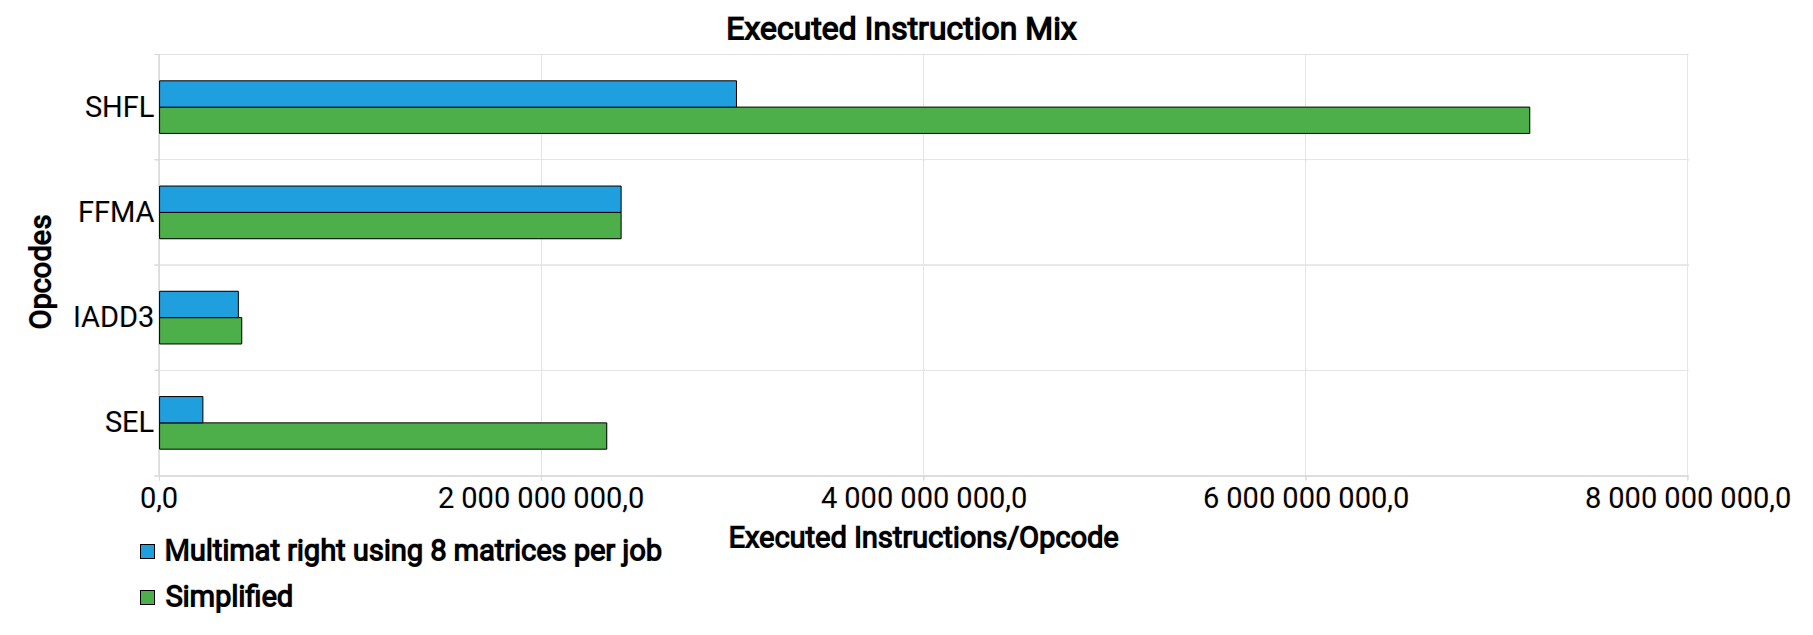
\includegraphics[width=\textwidth]{executed_instructions_multimat_right.png}
		\caption{Executed instruction mix.}
		\label{fig:executed_instructions_multimat_right}
	\end{subfigure}
	\hfill
	\begin{subfigure}{\textwidth}
		\centering
		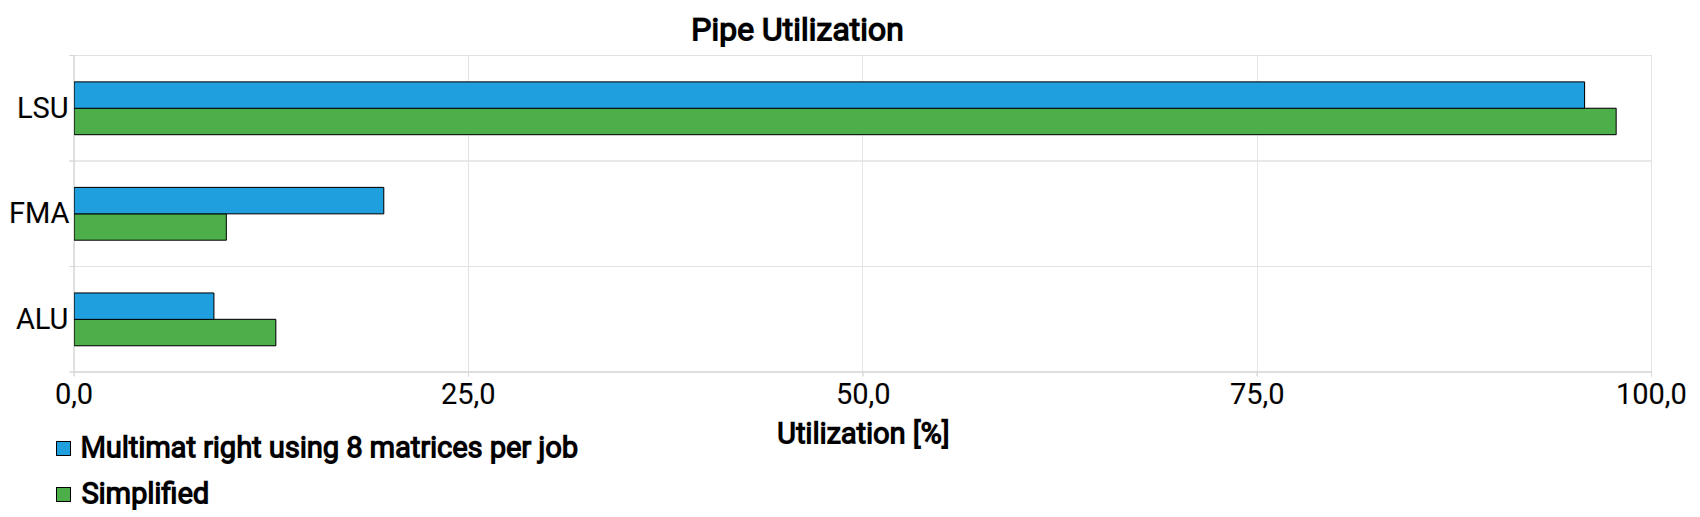
\includegraphics[width=\textwidth]{pipeline_utilization_multimat_right.png}
		\caption{Pipeline utilization.}
		\label{fig:pipeline_utilization_multimat_right}
	\end{subfigure}
	
	\caption{Comparison of \textit{one-to-many} simplified algorithm with the multiple right matrix optimization.}
	\label{fig:multimat_right_profiling}
\end{figure}

There are several ways to improve the ratio of SHFL instructions to FFMA instructions. The one with easiest changes to the code of the Simple warp shuffle implementation is to utilize the \textit{one-to-many} type of computation, and let each worker compute cross-correlation between one left matrix and many right matrices at once, as described in section \ref{sec:data_reuse_overlap} under the name \textit{multimat}. We call this exact implementation usable for \textit{one-to-many} and \textit{n-to-mn} types the \textit{multimat\_right} optimization, as each job contains multiple overlaps of a single left matrix with multiple right matrices. The obvious advantage is data reuse, as the data from the left matrix is used to compute multiple results. The main advantage is that each additional right matrix only adds a single SHFL instruction, while also adding one FFMA instruction. The ratio of SHFL to FFMA instructions can then be expressed as $2 + r : r$, where $r$ is the number of overlaps (from $r$ right matrices) computed by each worker, which for larger values of $r$ significantly improves the $3:1$ ratio of the simplified warp shuffle algorithm.


The code changes required to implement this are very straightforward, and can be found applied in the attachments of this thesis in the file \texttt{code/src/naive\_shuffle\_multimat\_right.cu} as the \texttt{ccn\_shuffle\_multimat\_right} kernel. Combination of this optimization and the \textit{work distribution} optimization described in Section \ref{sec:warp_shuffle_work_dist} can be found as the \texttt{ccn\_shuffle\_multimat\_right\_work\_distribution} in the same file.

As each job contains the same overlap between one left matrix and multiple right matrices, the three for loops and their bounds described in Section \ref{sec:simplified_warp_shuffle_steps} are left unchanged. The main difference is that the \textit{sum} and the \textit{thread\_right} variables in each thread are changed into arrays, utilizing the CUDA local array optimization described in Appendix \ref{sec:local_array_optimization}. This increases the amount of data present in registers and allows us to reuse data loaded from the left matrix with data from multiple right matrices. The code changes are illustrated in Listing \ref{lst:multimat_right_changes}.

\begin{lstlisting}[
style=cuda,
float,
caption=Changes for multimat right implementation,
label=lst:multimat_right_changes
]
template<size_t NUM_RIGHTS, typename T>
__device__ void warp_shuffle_multimat_right_impl(...) {
	...
	T sum[NUM_RIGHTS];
	for (size_t r = 0; r < NUM_RIGHTS; ++r) {
		sum[r] = 0;
	}
	...
	T thread_right[NUM_RIGHTS];
	for (size_t r = 0; r < NUM_RIGHTS; ++r) {
		thread_right[r] = load_with_bounds_check(...);
	}
	...
	for (dsize_t r = 0; r < NUM_RIGHTS; ++r) {
		// Broadcast right buffer
		auto right_val = warp.shfl(thread_right[r], i);
		sum[r] += thread_left_bottom * right_val;
	}
}
\end{lstlisting}

We introduce the term \textit{matrix group}, describing the right input matrices from which overlaps are grouped into a single job. As the size of the matrix group must be known at compile time to utilize the CUDA local array optimization, the \textit{device} function implementing the algorithm needs to be compiled for each supported matrix group size in the \texttt{NUM\_RIGHTS} template argument. This introduces a trade-off between compilation time, generated code size and the number of required registers on one hand and possible gains during run-time on the other. The actual matrix group size used during run-time is specified as run-time argument for the algorithm, which then chooses the correct implementation. If the number of matrices is not divisible by the matrix group size, the last few matrices will form a smaller matrix group which will choose the implementation based on its size. The maximum supported matrix group size is configurable during compile-time.

The number of thread blocks is increased to start enough workers to process all jobs. Threads of each thread block are assigned jobs from a single matrix group, again assigning jobs containing 32 consecutive overlaps in each output matrix of the matrix group to threads of a single warp. This allows us to reuse most of the Simple warp shuffle algorithm code.
% TODO: Maybe figure of job assignment to threads of a warp

The effects of this optimization shown in Figure \ref{fig:multimat_right_profiling}, which compares the simplified algorithm against the optimized algorithm using 8 right matrices grouped into a single job (which is a default maximum group size to keep compile times and executable size manageable) with input of size 256x256 with 1 left matrix and 16 right matrices, which are enough to saturate the RTX 2060 used for profiling. In this profiling, the \texttt{LSU} pipeline is still a bottleneck even for the optimized algorithm, but the utilization of the \texttt{FMA} pipeline, which does the useful part of the computation, has increased from 9\% to 20\%. The most visible change is in the mix of the executed instructions, where we see a very noticeable improvement in the ratio of shuffle instructions (SHFL) to the floating point fused multiply-add instructions (FFMA). As expected, the ratio improves from $3 : 1$ to $10 : 8$, with $3 019 898 880 : 2 415 919 104$ SHFL to FFMA instructions. The relatively small improvement in the \texttt{LSU} pipeline utilization can be explained by the low throughput of the SHFL instructions compared to the FFMA instructions. This is exacerbated by our use of Compute Capability 7.5 card for profiling, which has half the warp shuffle throughput of all other Compute Capabilities.

\subsection{Multiple rows from the right matrix}
\label{sec:multirow_right}

Another way to improve the instruction ratio is to process multiple overlaps from the same output matrix, which can be used even for the \textit{one-to-one} type of computation. We call this the \textit{multirow\_right} optimization, as we compute overlaps from multiple consecutive rows of a single column of the output matrix as shown in Figure \ref{fig:multirow_shifts}, where we see two different jobs, each containing 4 overlaps, i.e. \textit{job\_size} is 4. We call it \textit{multirow\_right} as it loads multiple rows from the right matrix at once to compute the assigned overlaps. This optimization provides us a different way to improve the ratio of warp shuffle to fused multiply-add instructions, independent of the changes in \textit{multimat\_right}. Thanks to this it can be combined with \textit{multimat\_right}. It is not however able to be combined with the \textit{work distribution} optimization. The code of this optimization can be found in the attachments of this thesis in the file \texttt{code/src/naive\_shuffle\_multirow\_right.cu} as the \texttt{ccn\_shuffle\_multirow\_right} kernel. 


\begin{figure}[ht]
	\centering
	\def\svgwidth{0.6\textwidth}
	\fontsize{6}{8}\selectfont
	% Must be relative to current directory
	% as input ignores graphicspath, which is
	% only for includegraphics{}
	\input{./img/overlap-Multirow.pdf_tex}
	\caption{Overlaps grouped into two different jobs by the \textit{multirow\_right} algorithm with 4 overlaps per job.}
	\label{fig:multirow_shifts}
\end{figure}

The core of the implementation is similar to the simplified algorithm. We compute the warp submatrix of the right input matrix containing all elements used by any of the overlaps in jobs assigned to the threads in the given warp. We then iterate over this submatrix, computing all \textit{job\_size} overlaps in a single pass. This reduces parallelism, as simplified algorithm would have split these overlaps into different jobs and computed them in parallel, but allows for data reuse, which is advantageous when the GPU is already saturated.

As each overlap in a given job has different shift in the \textit{y} axis, each overlap will contain different number of rows as shown in Figure \ref{fig:multirow_shifts}, but thanks to the column-wise grouping of overlaps, corresponding overlaps in each job assigned to threads of a single warp will contain the same group of rows. This again allows us to reuse much of the simplified implementation code, which expects a warp to process overlaps with the same number of rows.

The problem experienced by this optimization is in its nature similar to the one shown in the Simple Warp shuffle implementation, where some of the threads need to execute the first few and the last few iterations of the innermost loop by adding zero to their sum thanks to bound checked loads. This is caused by the different shifts of the overlaps assigned to threads of a single warp, where some of the overlaps do not use whole warp submatrix, which contains input data used by any of the overlaps assigned to the threads of the warp.

As we now group several overlaps into a single job computed by a single thread, the same problem arises where only a subset of the overlaps has the first few rows and last few rows of the warp submatrix as inputs. More precisely, some of the first $0$ to $job\_size - 1$ and the last $0$ to $job\_size - 1$ rows are only required by some of the overlaps assigned to the given thread, and as all threads of a warp are assigned overlaps from the same rows of the output matrix in 32 consecutive columns, the subset of overlaps to which each row of warp submatrix is an input is the same for all threads of a warp.

To solve this problem, we split the outermost loop going over the rows of the warp submatrix into three parts. First few iterations are separated into \textit{Init} iterations, which compute only the subset of overlaps which actually require the rows of the warp submatrix as input. Then we have the \textit{Main loop}, which computes all overlaps assigned to the thread. Lastly we have several \textit{Finish} iterations, which again compute only the subset of overlap which require the given warp submatrix row as input. This partitioning is illustrated in Figure \ref{fig:multirow_right_steps}. The number of \textit{Init} and \textit{Finish} steps depends on the exact shift of the overlaps grouped into a job.

Code changes for this implementations are similar to the changes for the \textit{multimat\_right} from Section \ref{sec:multimat_right}, again using Local array optimization described in Appendix \ref{sec:local_array_optimization}. We again compute multiple results in each thread, iterating over multiple rows from a single right matrix where \textit{multimat\_right} loaded the different rows from multiple separate right matrices. The only other major change is the partitioning of the outermost loop as described above. The similarity of the changes is utilized when combining  \textit{multirow\_right} and \textit{multimat} optimizations.

\begin{figure}[ht]
	\centering	
	\begin{subfigure}{\textwidth}
		\centering
		\def\svgwidth{\textwidth}
		% Must be relative to current directory
		% as input ignores graphicspath, which is
		% only for includegraphics{}
		\input{./img/overlap-MultirowInit.pdf_tex}
		\caption{Complete computation of the \textit{multirow\_right} algorithm with \textit{job\_size} 3 for overlaps with shifts $[1, 1], [1, 2], [1, 3]$ showcasing Init steps.}
		\label{fig:multirow_init}
	\end{subfigure}
	\hfill
	\begin{subfigure}{\textwidth}
		\centering
		\def\svgwidth{\textwidth}
		% Must be relative to current directory
		% as input ignores graphicspath, which is
		% only for includegraphics{}
		\input{./img/overlap-MultirowFinalize.pdf_tex}
		\caption{Complete computation of the \textit{multirow\_right} algorithm with \textit{job\_size} 3 for overlaps with shifts $[1, -3], [1, -2], [1, -1]$ showcasing Finish steps}
		\label{fig:multirow_fini}
	\end{subfigure}
	
	\caption{Illustration of Init and Finish steps of the \textit{multirow\_right} algorithm with overlaps processed in each step displayed above the step.}
	\label{fig:multirow_right_steps}
\end{figure}



One of the disadvantages of this algorithm is the repeated reading of right input matrix rows by each worker. As warp shuffle is already utilized for data reuse in the given row, there is no simple mechanism to reuse data between rows as we traverse the warp submatrix from top to bottom. With 3 overlaps grouped into a job, each row of the right input matrix processed by the main loop is read 3 times by the worker, once for each of the overlaps assigned to the worker. Each time, it is used with different left row. This can be improved by also utilizing multiple rows from the left input matrix, computing multiple iterations of the current main loop at once. This implementation, named \textit{multirow\_both} as we read multiple rows in each iteration from both input matrices, is described in Section \ref{sec:multirow_both}.


When profiling this optimization, as shown in Figure \ref{fig:multirow_right_profiling}, we see similar improvements as with the previous \textit{multimat\_right} optimization. We have to keep in mind that the \textit{multirow\_right} algorithm improves the \textit{one-to-one} type of computation, which cannot be improved by the previous optimization. These two optimizations can also be combined, which is described in Section \ref{sec:combining_optimizations}. As before, the \textit{LSU} pipeline remains a bottleneck, but the utilization of \textit{FMA} pipeline is improved from 9\% to 17\%. With 4 overlaps per job, the ratio improves from $3 : 1$ to $6 : 4$ as expected from the $2 + r : r$ theoretical ratio with $227 367 936 : 150 994 944$ SHFL to FFMA instructions. As this optimization improves the \textit{one-to-one} computation, it is more sensitive to occupancy reduction when workers process more than one overlap, mainly due to the smaller input size compared to the \textit{one-to-many} computation.

\begin{figure}[ht]
	\centering	
	\begin{subfigure}{\textwidth}
		\centering
		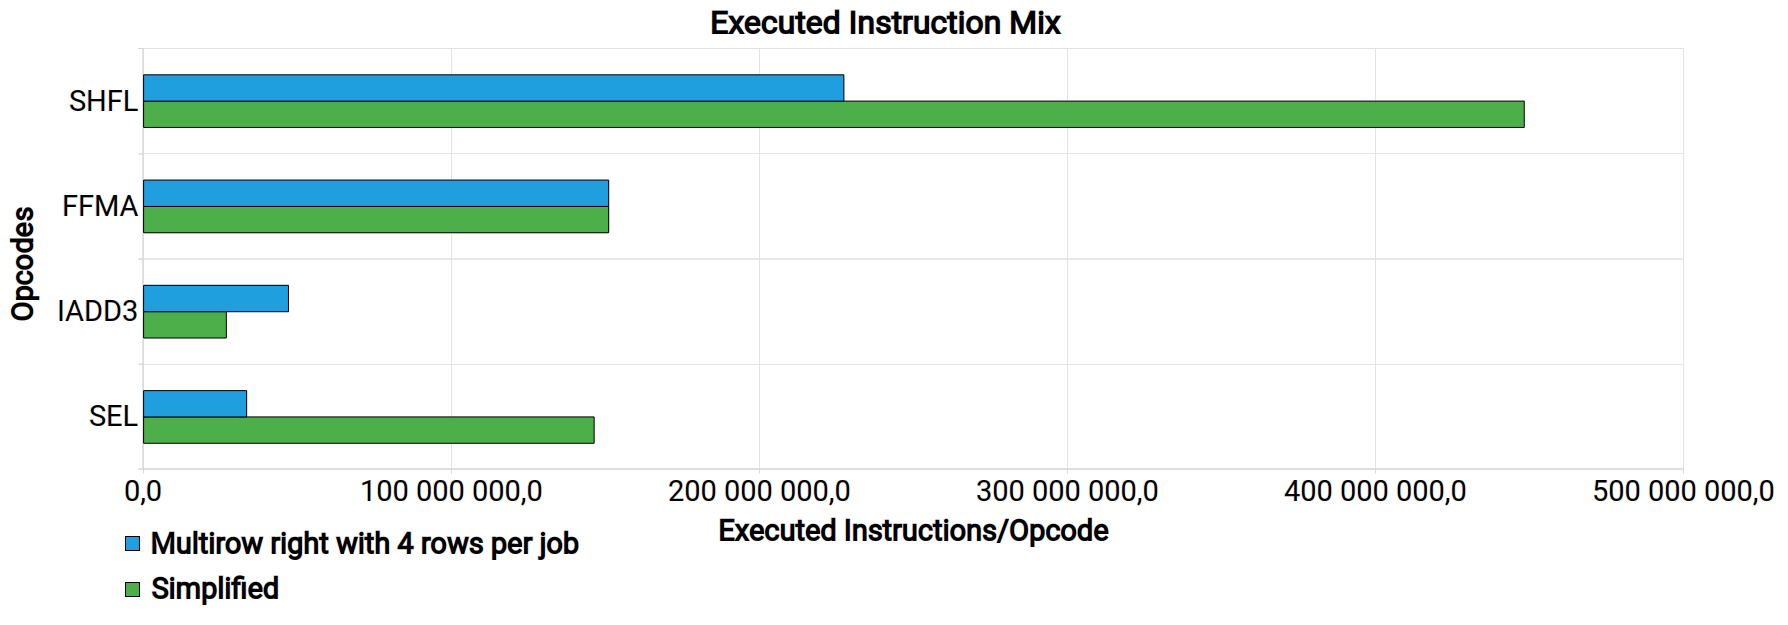
\includegraphics[width=\textwidth]{executed_instructions_multirow_right.png}
		\label{fig:executed_instructions_multirow_right}
	\end{subfigure}
	\hfill
	\begin{subfigure}{\textwidth}
		\centering
		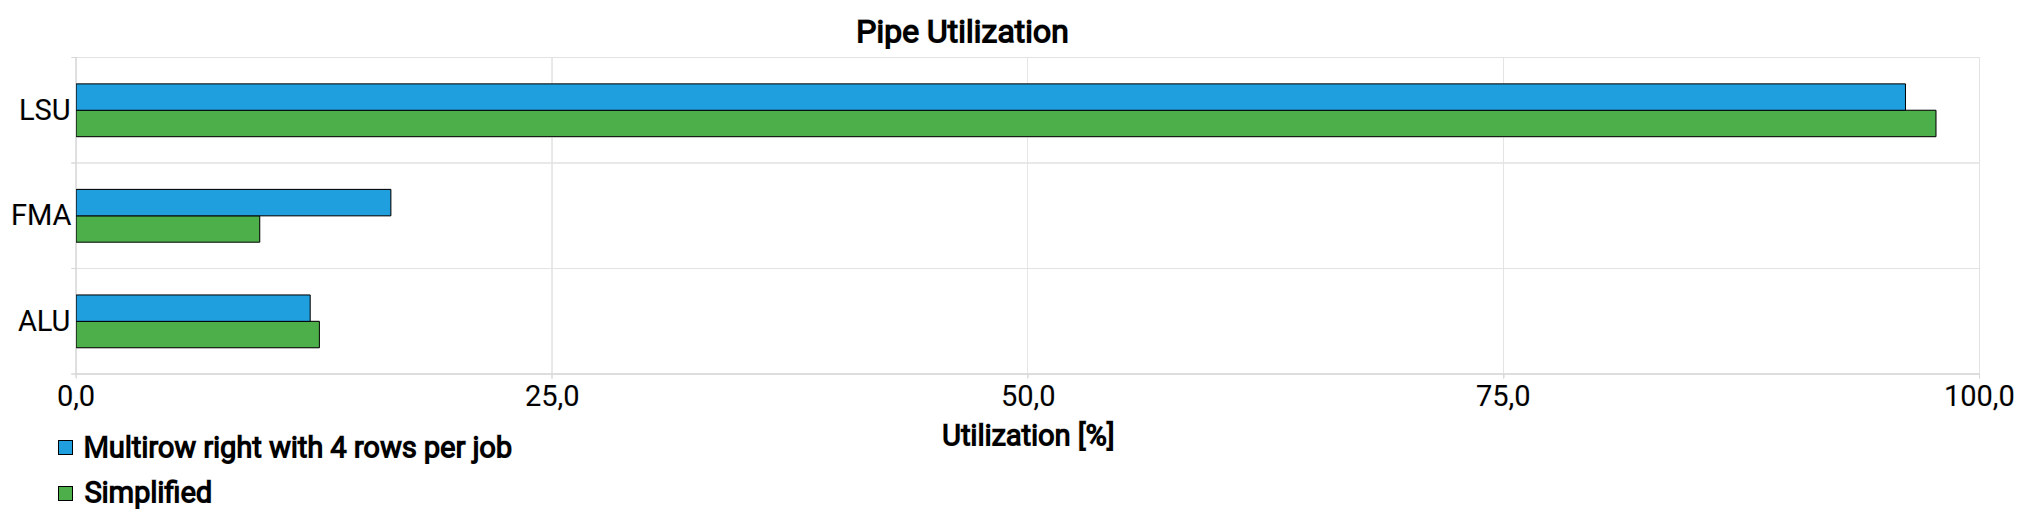
\includegraphics[width=\textwidth]{pipeline_utilization_multirow_right.png}
		\label{fig:pipeline_utilization_multirow_right}
	\end{subfigure}
	
	\caption{Comparison of \textit{one-to-one} simplified algorithm with the \textit{multirow\_right} optimization.}
	\label{fig:multirow_right_profiling}
\end{figure}

% TODO: Computing with double

\subsection{Multiple left matrices}
\label{sec:multimat_both}

This optimization is an extension of the \textit{multimat\_right} aiming at the reuse of data from the right input matrix to compute cross-correlation with multiple left input matrices. As we now reuse data from both left and right input matrices, we call this the \textit{multimat\_both} optimization. This optimization is only usable for the \textit{n-to-m} computation type, as the \textit{one-to-one}, \textit{one-to-many}, and \textit{n-to-mn} types correlate each left matrix with a different set of right matrices.

Similarly to the \textit{multimat\_right} optimization, we group overlaps represented by elements at the same index in multiple output matrices into a single job. These overlaps represent the same shift between the input matrices, with each representing an overlap of a different pair of input matrices. Whereas the \textit{multimat\_right} output matrices represented cross-correlation between a single left input matrix and multiple right matrices, with \textit{multimat\_both} the output matrices represent cross-correlations of the \textit{n-to-m} (\textit{all-to-all}) type between multiple left and multiple right matrices, as explained in Section \ref{sec:data_reuse_overlap}

The implementation of this optimization can be found in the attachments of this thesis in the file \texttt{code/src/naive\_shuffle\_n\_to\_m\_multimat\_both.cu} in the \texttt{ccn\_shuffle\_n\_to\_m\_multimat\_both\_work\_distribution}. As the name suggests, this optimization can be combined with the \textit{work distribution} optimization. To measure the performance without work distribution, we use the \textit{None} distribution type described in Section \ref{sec:warp_shuffle_work_dist}.


The changes to the \textit{multimat\_right} optimization code to implement \textit{multimat\_both} again utilize the Local array optimization described in Appendix \ref{sec:local_array_optimization}, changing the variable representing the left buffer in each thread into an array representing multiple buffers. 


Similarly to the \textit{multimat\_right} optimization, we group input matrices into matrix groups, this time separately grouping left matrices into \textit{left\_matrix\_groups} and right matrices into \textit{right\_matrix\_groups}. Each pairing of $l$ left matrix group with $r$ right matrix group defines a set of $l*r$ output matrices due to the \textit{n-to-m} computation type. Elements in column $x$ and row $y$ from all of these $l*r$ matrices are grouped into a single job, computed by a single thread. 

The number of matrices in a left matrix group is configured independently of the number of matrices in a right matrix groups. The maximum size of left matrix group and right matrix group has to be known at compile time so that we can generate the implementing device function for all combinations of these values from 1 to the configured maximum, as the arrays must have a size known at compile time. At run-time, the implementation chooses the correct method. The last matrix groups from both left and right input matrices may be smaller as the number of left or right matrices may not be divisible by the value of the run-time argument. The implementation then chooses the function with the correct matrix group size, which is why we must generate the implementing function for possible matrix group sizes.

For each pairing of left matrix group and right matrix group, we start enough thread blocks to process all jobs defined by this pair of thread groups. Threads of a single thread block process jobs from a single pairing of left matrix group and right matrix group. This again allows us to minimize the required changes to the code of \textit{multimat\_right} optimization when implementing \textit{multimat\_both}.


The \textit{multimat\_both} optimization can be combined with either \textit{work distribution} or \textit{multirow\_right} optimizations. It can also be combined with \textit{multirow\_both} optimization introduced in the following section.


% TODO: unused workers
% TODO: Separate covering of an output matrix from each group

This optimization improves the ratio of warp shuffle (SHFL) to fused multiply-add (FFMA) instructions to $ 2 * l + r : l * r$, where $l$ is the number of left matrices in the left matrix group and $r$ the number of right matrices in the right matrix group. This is to be compared to the $3:1$ ratio of the Simple warp shuffle implementation, $2 + r : r$ of the \textit{multimat\_right} optimization, and slightly worse than $2 + r : r$ \textit{multirow\_right} with $r$ representing number of rows instead of matrices grouped into a single job. As with these previous optimizations, this improvement comes at the cost of parallelism, as all overlaps grouped into a single job would be executed in parallel without this optimization. For larger input matrices and larger numbers of input matrices, this reduction in parallelism is more than compensated by the improved throughput of each thread thanks to the improved instruction ration. For smaller input sizes, the reduction in parallelism can be compensated for by combining this optimization with \textit{work distribution} optimization.



The ratio of SHFL to FFMA instructions is shown in Figure \ref{fig:multimat_both_executed_instructions}. The profiling was executed with both matrix group sizes set to 4 on input of 4 left matrices and 16 right matrices of size 256x256 elements. The expected ratio is $12 : 16$, which is exactly what we see in the measurements with $7 247 757 312 : 9 663 676 416$ SHFL to FFMA instructions. This improved ratio also results in improved utilization of the FMA pipeline, which is now utilized to
$31.2\%$ of its maximum throughput. Comparison of the effects on execution time is provided in Section \ref{sec:results_definition_based}.

\begin{figure}
	\centering
	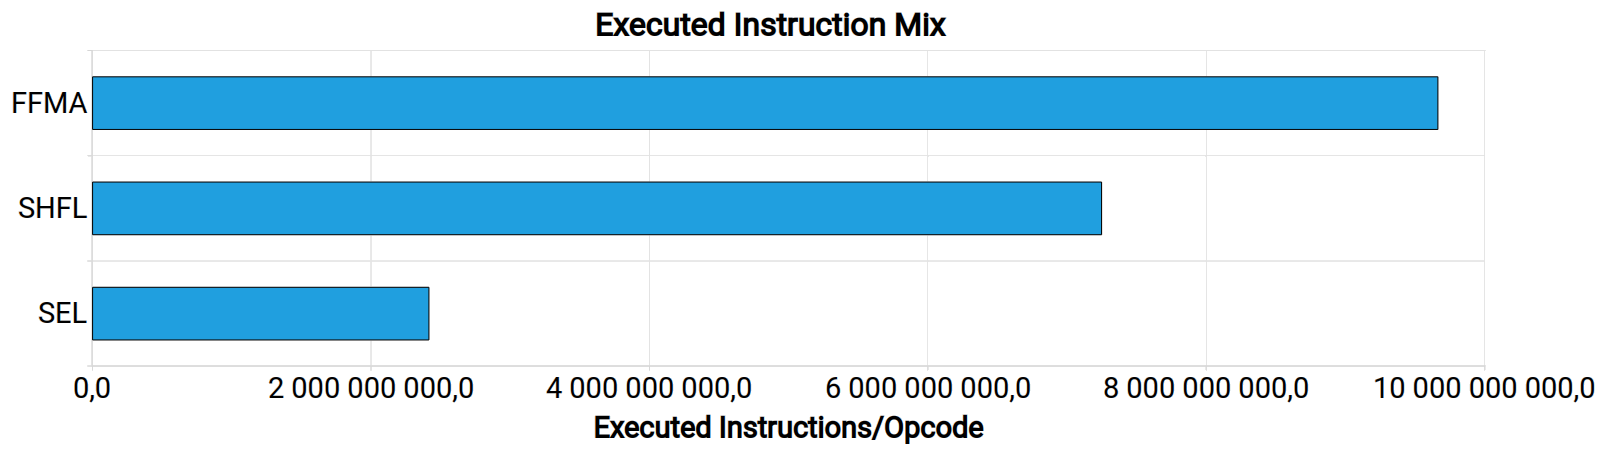
\includegraphics[width=\textwidth]{executed_instructions_multimat_both.png}
	\caption{Three most often executed instructions by the Warp shuffle algorithm with \textit{multimat\_both} optimization.}
	\label{fig:multimat_both_executed_instructions}
\end{figure}


\subsection{Multiple rows from both matrices}
\label{sec:multirow_both}

When improving the \textit{one-to-one} computation using the \textit{multirow\_right} optimization described in Section \ref{sec:multirow_right}, which processes multiple overlaps from consecutive rows of a single column of the output matrix, we hinted at a further improvement using multiple rows from the left matrix in the main loop. This not only improves the ratio of warp shuffle to fused multiply-add instructions, but also reduces the number of times every row from the right input matrix is read. 

The main change to the code of \textit{multirow\_right} optimization is that the main loop now advances by multiple left input matrix rows instead of a single row. This new implementation can be found in the attachments of this thesis in the file \texttt{code/src/naive\_shuffle\_multirow\_both.cu} as the \texttt{ccn\_shuffle\_multirow\_both} kernel.

The exact number of left rows to advance by in each iteration is configured by an algorithm argument. An additional stage between this multistep main loop and Finish is also needed to compute the remaining rows from the left input matrix when the total number of left input matrix rows is not divisible by the main loop step. This stage utilizes the original single step main loop. The Init and Finish parts are left unchanged.



The ratio of warp shuffle instructions (SHFL) to fused multiply-add instructions (FFMA) for this optimization is $l + (o - 1 + l) : l * o$ in the main loop, where $l$ is the number of left rows processed by each iteration of the main loop and $o$ is the number of overlaps grouped into a single job.  
The Init, single step main loop and Finish parts share the original ratio of the \textit{multirow\_right} implementation, which is $2 + o : o$. This ratio is also apparent in Figure \ref{fig:multirow_both_executed_instructions}. The profiling is done for cross-correlation of two 256x256 matrices with both number of left rows per iteration $l$ and number of overlaps grouped into a job $o$ set to 4. The expected ratio of SHFL to FFMA instructions is $11:12$, which is almost exactly what we see with $140 006 752 : 150 994 994$ total SHFL to FFMA instructions. This improved ratio also results in additional utilization of the FMA pipeline, which utilizes $23.9\%$ of its total throughput, compared to $10\%$ utilization by the Simple warp shuffle implementation and $17\%$ by \textit{multirow\_right} optimization.

\begin{figure}
	\centering
	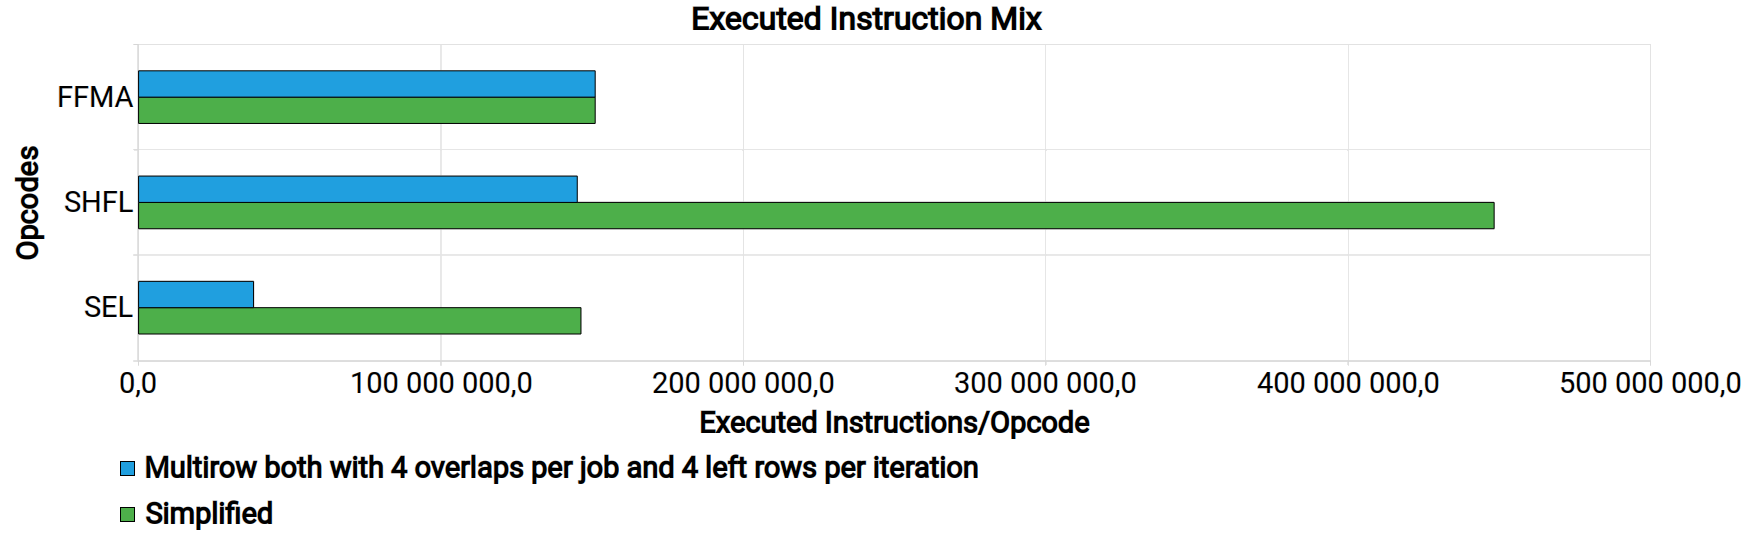
\includegraphics[width=\textwidth]{executed_instructions_multirow_both.png}
	\caption{Three most often executed instructions by the Warp shuffle algorithm with \textit{multirow\_both} optimization.}
	\label{fig:multirow_both_executed_instructions}
\end{figure}


\subsection{Summary}
\label{sec:combining_optimizations}

In this section, we have implemented a family of Warp shuffle based implementations with the following optimizations:
\begin{itemize}
	\item \textit{work distribution} (Section \ref{sec:warp_shuffle_work_dist}),
	\item \textit{multimat\_right} (Section \ref{sec:multimat_right}),
	\item \textit{multirow\_right} (Section \ref{sec:multirow_right}),
	\item \textit{multimat\_both} (Section \ref{sec:multimat_both}),
	\item \textit{multirow\_both} (Section \ref{sec:multirow_both}).
\end{itemize}

The Warp shuffle family utilizes warp shuffle instructions to reuse data already loaded into registers by multiple threads of a warp, reducing the required number of load operations from global memory. The optimizations then improve occupancy through splitting work into smaller jobs, improve ratio of warp shuffle instructions to fused multiply-add instructions or improve data reuse once loaded into registers.


The \textit{work distribution}, \textit{multimat\_right}, and \textit{multirow\_right} are implemented by improving the Simple warp shuffle implementation. The  \textit{multimat\_both} and \textit{multirow\_both} optimizations are implemented as extensions to the \textit{multimat\_right} and \textit{multirow\_right} optimizations respectively.


All of the optimizations listed above can be combined with the following restrictions:
\begin{enumerate}
	\item \textit{multirow} optimizations cannot be combined with work distribution,
	\item \textit{multimat\_both} can only be used to optimize the \textit{n\_to\_m} computation. 
\end{enumerate}

With the \textit{multirow} optimization, each job contains several different overlaps of the two input matrices, where each overlap has different number of rows. As our work distribution optimization is based on the number of rows of the overlap, the current implementation cannot be easily reused. This is not a problem with the \textit{multimat} optimizations, in which each thread computes the same overlap in multiple output matrices.

The \textit{n\_to\_m} computation type is the only type where multiple left matrices share the same right matrix, which makes it possible to reuse the data from the left matrices.


With these restrictions in mind, we have implemented the following versions of the warp shuffle algorithm:

% TODO: Maybe change into a table with matching implemented calculation types
\begin{itemize}
	\item multimat\_right,
	\item multimat\_right\_work\_distribution,
	\item multimat\_both\_work\_distribution,
	\item multirow\_right,
	\item multirow\_right\_multimat\_right,
	\item multirow\_both,
	\item multirow\_both\_multimat\_right,
	\item multirow\_both\_multimat\_both.
\end{itemize}

Both \textit{multimat} optimizations were already prepared for combination with work distribution, as hinted at in their respective sections. The core computation code does not change, the only difference is that we split the original warp submatrix the same way we did when implementing work distribution for simplified warp shuffle algorithm, described in Section \ref{sec:warp_shuffle_work_dist}.

Combination of \textit{multimat} and \textit{multirow} optimizations takes the implementation of \textit{multimat} optimization, separates the middle and inner loop as is done to the simplified implementation in the implementation of \textit{multirow} and splits the outer loop iterations into Init, multistep main loop, single step main loop, and Finish parts.

The measurement and comparison of these implementations is presented in Section \ref{sec:results_definition_based}.

\section{Warp per shift algorithm family}
\label{sec:warp_per_shift}

% REFERENCE file:///home/karel/skola/diplomka/crosscorr/papers/related_work/levenstein.pdf and their choice of size

For small inputs, processing a single overlap or a row group per thread may not split the computation into enough jobs to saturate the whole GPU, leading to low occupancy. As described in Section \ref{sec:occupancy}, low occupancy prevents the full utilization of the throughput of the GPU hardware, while also preventing the GPU from hiding the high latency of each instruction, resulting in poor performance. To increase the number of threads started for smaller inputs, we increase the size of each worker from a single thread to a whole warp. This increase in number of threads in combination with the small input data size leads to a need of balancing the overhead of each thread, which consists mainly of scheduling, repeated data reads, and computation of array indexes for each access, with the reduced workload. 

%For each implementation, there exists an input size for which the overhead results in pure CPU based implementation being faster than the GPU implementation. This bound is specific to each system, as it is based on the relative power of the CPU and GPU, together with the interconnection between GPU and CPU for data transfer. This topic is further explored in Section \ref{sec:warp_per_shift_vs_cpu}.

In this section, we first introduce a base implementation of the \textit{warp per shift} algorithm utilizing whole warps as workers with each job containing a single overlap, also called shift. We then introduce several improvements of this algorithm, first by using shared memory and then by further increasing the number of jobs using work distribution optimization

This algorithm family is inspired by \citet{paper:levenstein}, who also choose to assign their unit of work to larger groups in the CUDA thread hierarchy. The work presents two implementations, first one where each stripe (their unit of work) is processed by a single warp which exchange data through warp shuffle instructions, which inspired our Warp shuffle algorithm family presented in Section \ref{sec:warp_shuffle_alg}. The warp per shift algorithm family described in this section is based on the second implementation where each strip is processed by a whole thread block with threads exchanging data using shared memory. 

In this section, we first introduce a base implementation assigning each element of the output matrix to a separate warp without any cooperation between warps. We then take inspiration from \citet{paper:levenstein} and use shared memory to cache input data used by warps of each thread block. We then further increase the number of jobs using work distribution optimization, adapted from the implementation described in Section \ref{sec:warp_shuffle_work_dist}. 

\subsection{Base implementation}



Implementation of the \textit{Warp per shift} algorithm is very simple compared to the warp shuffle-based algorithm described in Section \ref{sec:warp_shuffle_alg}. The basic implementation utilizes whole warps as workers and assigns each worker a job consisting of a single overlap. Each overlap is uniquely identified by the shift of the two input matrices, and the shift is what is stored and propagated throughout the code. This is why we call this the \textit{warp per shift} algorithm family.

\begin{figure}[ht]
	\centering	
	\begin{subfigure}{0.55\textwidth}
		\fontsize{6}{8}\selectfont
		\centering
		\def\svgwidth{\textwidth}
		% Must be relative to current directory
		% as input ignores graphicspath, which is
		% only for includegraphics{}
		\input{./img/overlap-Shifts.pdf_tex}
		\caption{Output matrix and the corresponding overlaps.}
		\label{fig:warp_per_shift_overlaps}
	\end{subfigure}
	\hfill
	\begin{subfigure}{0.4\textwidth}
		%\fontsize{6}{8}\selectfont
		\centering
		\def\svgwidth{\textwidth}
		\fontsize{6}{8}\selectfont
		% Must be relative to current directory
		% as input ignores graphicspath, which is
		% only for includegraphics{}
		\input{./img/overlap-WarpPerShiftWarps.pdf_tex}
		\caption{Distribution of overlaps in a 3 by 7 output matrix between thread blocks and their warps.}
		\label{fig:warp_per_shift_warps}
	\end{subfigure}
	
	\caption{Output matrix and its distribution between warps.}
\end{figure}

As in the Basic cross-correlation algorithm, introduced in Section \ref{sec:basic_alg}, this implementation uses two dimensional grid of two dimensional thread blocks to assign elements of the output matrix to workers. The difference is in how we use each dimension to map threads to overlaps, this time based on which warp and thread block they are part of. All threads of a warp are assigned the same overlap and they cooperate to compute all the tasks (yellow boxes) which belong to this overlap. The mapping from thread blocks and warps to overlaps of the output matrix is illustrated by Figure \ref{fig:warp_per_shift_warps}. Warps of each thread block are assigned consecutive overlaps in a row of the output matrix. The number of warps per thread block is configurable by algorithm argument.

Each thread of a warp is assigned subset of the multiplication tasks (yellow boxes), as shown in Figure \ref{fig:warp_per_shift_normal_indexing}, which it computes and holds the sum in local variable. This distribution is done using the code in Listing \ref{lst:warp_per_shift_base}, which is a snippet of the kernel \texttt{ccn\_warp\_per\_shift} found in the file \texttt{code/src/naive\_warp\_per\_shift.cu} in thesis attachments.

\begin{lstlisting}[
style=cuda,
float,
caption=Main loop of the Base Warp per shift implementation,
label=lst:warp_per_shift_base
]
for (
	size_t i = warp.thread_rank(); 
	i < total_items; 
	i += warp.size()
) {
	size_t overlap_row = i / overlap_size.x;
	size_t overlap_row_offset = i % overlap_size.x;

	size_t right_idx = ...;
	size_t left_idx = ...;

	sum += left[left_idx] * right[right_idx];
}
\end{lstlisting}

\begin{figure}[ht]
	\centering
	\def\svgwidth{0.5\textwidth}
	\fontsize{8}{10}\selectfont
	% Must be relative to current directory
	% as input ignores graphicspath, which is
	% only for includegraphics{}
	\input{./img/warp_per_shift-Basic.pdf_tex}
	\caption{Thread computing given task with basic indexing (example warp size 4).}
	\label{fig:warp_per_shift_normal_indexing}
\end{figure}

This distribution of tasks minimizes thread divergence but may lead to uncoalesced global memory access. Another possible disadvantage of this implementation is the division and the modulo instruction in each loop iteration, which is used to determine the position in the overlapping submatrix to be computed by the current thread.

% REFERENCE file:///home/karel/skola/diplomka/crosscorr/papers/related_work/Honz%C3%A1tko-Kruli%C5%A12019_Article_AcceleratingBlock-matchingAnd3.pdf where in section 5.1.1 threads of a warp cooperate to compute results
The distribution is based on the cooperative distance calculations by \citet{paper:krulis_3d_block}. In their work, warps of a thread cooperate to compute distance between neighboring overlapping patches of an image. Each thread computes a subset of columns and stores the results to shared memory. After all threads compute their assigned columns, each thread picks the results corresponding to its assigned patch. 

Our base warp per shift implementation utilizes slightly easier approach. Instead of assigning columns, the whole overlapping part of the input matrices is serialized in row major order and iterated over using the for loop illustrated above. 

The sums computed by each thread of the warp are then combined using the \texttt{cooperative\_groups::reduce} function, which may even be hardware accelerated if running on the newest Ampere GPUs. The final result is then written by thread with warp rank $0$ to the output matrix. 


\subsection{Simplified indexing}
\label{sec:simplified_indexing}

The Simplified indexing is an attempt to solve the problems highlighted in the previous section, namely the uncoalesced global memory access and the low throughput division instruction in the main loop. To fix these problems, we change the distribution of tasks between threads as shown in Figure \ref{fig:warp_per_shift_simplified_indexing}, which is much closer to the task distribution done by \citet{paper:krulis_3d_block}, but still not exactly the same. Compared to their implementation, each row of the overlap is processed independently and fully before continuing to the next row. Code of this implementation can be found in the attachments of this thesis in the file \texttt{code/src/naive\_warp\_per\_shift.cu} as the \texttt{ccn\_warp\_per\_shift\_simple\_indexing} kernel.

Compared to Basic indexing described in the previous section, this assures coalesced access to the global memory, but leads to thread divergence if the row size of the overlap is not a multiple of warp size, as is the case in Figure \ref{fig:warp_per_shift_simplified_indexing}. 

\begin{figure}[ht]
	\centering
	\def\svgwidth{0.5\textwidth}
	\fontsize{8}{10}\selectfont
	% Must be relative to current directory
	% as input ignores graphicspath, which is
	% only for includegraphics{}
	\input{./img/warp_per_shift-SimplifiedIndexing.pdf_tex}
	\caption{Comparison of task assignment with basic and simplified indexing (example warp size 4).}
	\label{fig:warp_per_shift_simplified_indexing}
\end{figure}

Thread divergence is the major problem of this implementation. Based on our profiling, the simplified indexing leads to an average of only 15.31 of the 32 threads executing each instruction and not being predicated (masked by a predicate). With basic indexing on the same input and on the same hardware, this average improves to 26.85, which is almost twice the work done per instruction. The main reason for this difference is shown in Figure \ref{fig:warp_per_shift_thread_divergence}. This figure shows the worst case scenario, where simplified indexing leads to the rows being processed sequentially, whereas basic indexing executes this in a single iteration. Overlaps such as this make up a sizable part of every cross-correlation computation. For larger input matrix sizes, the proportion of overlaps such as the ones shown in Figure \ref{fig:warp_per_shift_thread_divergence} which should increase the average of threads which are not masked during instruction execution, but based on our measurements in Section \ref{sec:results_occupancy_improvements}, simplified indexing does not improve execution time for inputs where increased occupancy due to the warp per shift algorithm family is more advantageous than the reduced number of global memory accesses by Warp shuffle family.

\begin{figure}[ht]
	\centering
	\def\svgwidth{0.45\textwidth}
	\fontsize{8}{10}\selectfont
	% Must be relative to current directory
	% as input ignores graphicspath, which is
	% only for includegraphics{}
	\input{./img/warp_per_shift-ThreadDivergence.pdf_tex}
	\caption{Task assignment with basic and simplified indexing to showcase thread divergence when using simplified indexing.}
	\label{fig:warp_per_shift_thread_divergence}
\end{figure}

One possible cause is that even though simplified indexing should theoretically lead to better coalescing of global memory access, the opposite seems to be the case as illustrated by Figure \ref{fig:executed_instructions_simplified_indexing}. This may be highly dependent on Compute Capability of the underlying hardware, but on CC 7.5 of RTX 2060, we observe a 47\% increase in the number of global memory requests when using simplified indexing. This corresponds to high \textit{LSU} pipeline usage of 88\% visible in Figure \ref{fig:pipeline_utilization_simplified_indexing}, which becomes a bottleneck. The profiling was done on input matrices of size 64 by 64 containing 32bit floating point numbers. In these matrices, each row is 256B long. In many overlaps, the last item of each row will be less than 128B (global memory transaction size) from the first item in the next row. This leads to coalescing of the global memory read with basic indexing but results in 2 separate accesses with simplified indexing, which may explain the 47\% difference in global memory requests.

Another visible difference in Figure \ref{fig:executed_instructions_simplified_indexing} is the increase in number of instructions across the board, most visible with branching (BRA) and barrier synchronization (BSYNC) instructions. This is caused by the increase in number of iterations each warp executes to process the same data. Even with the increase in number of instructions, the \textit{ALU} and \textit{FMA} pipelines are less utilized than with basic indexing. This is caused by warps waiting for warp recombination on the barrier synchronization points and loads from global memory.


\begin{figure}[ht]
	\centering	
	\begin{subfigure}{0.8\textwidth}
		\centering
		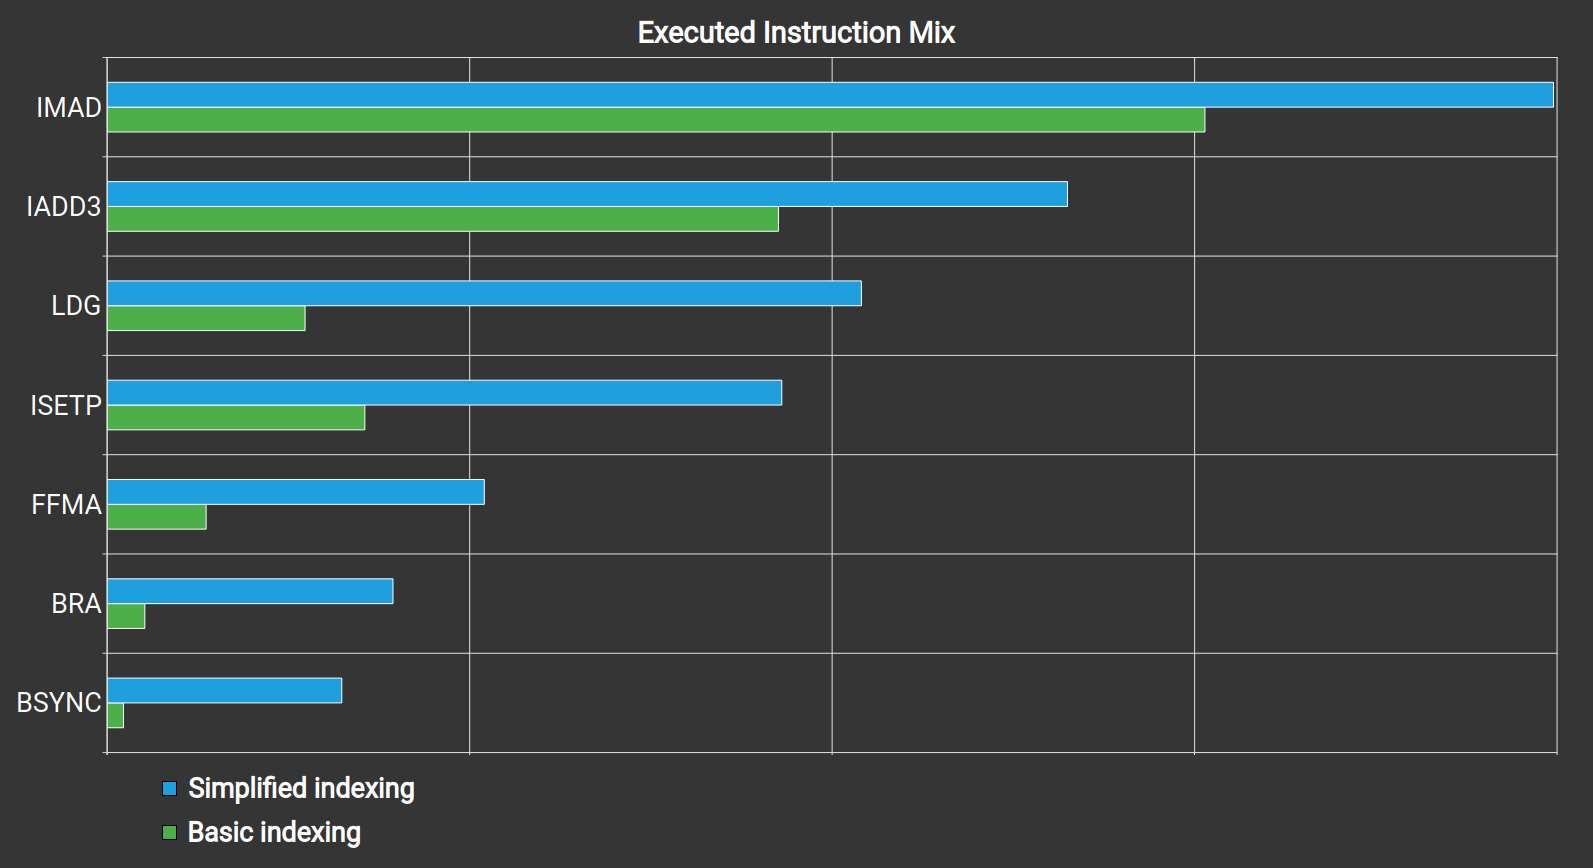
\includegraphics[width=\textwidth]{executed_instructions_simplified_indexing.png}
		\caption{Executed instruction mix.}
		\label{fig:executed_instructions_simplified_indexing}
	\end{subfigure}
	\hfill
	\begin{subfigure}{0.8\textwidth}
		\centering
		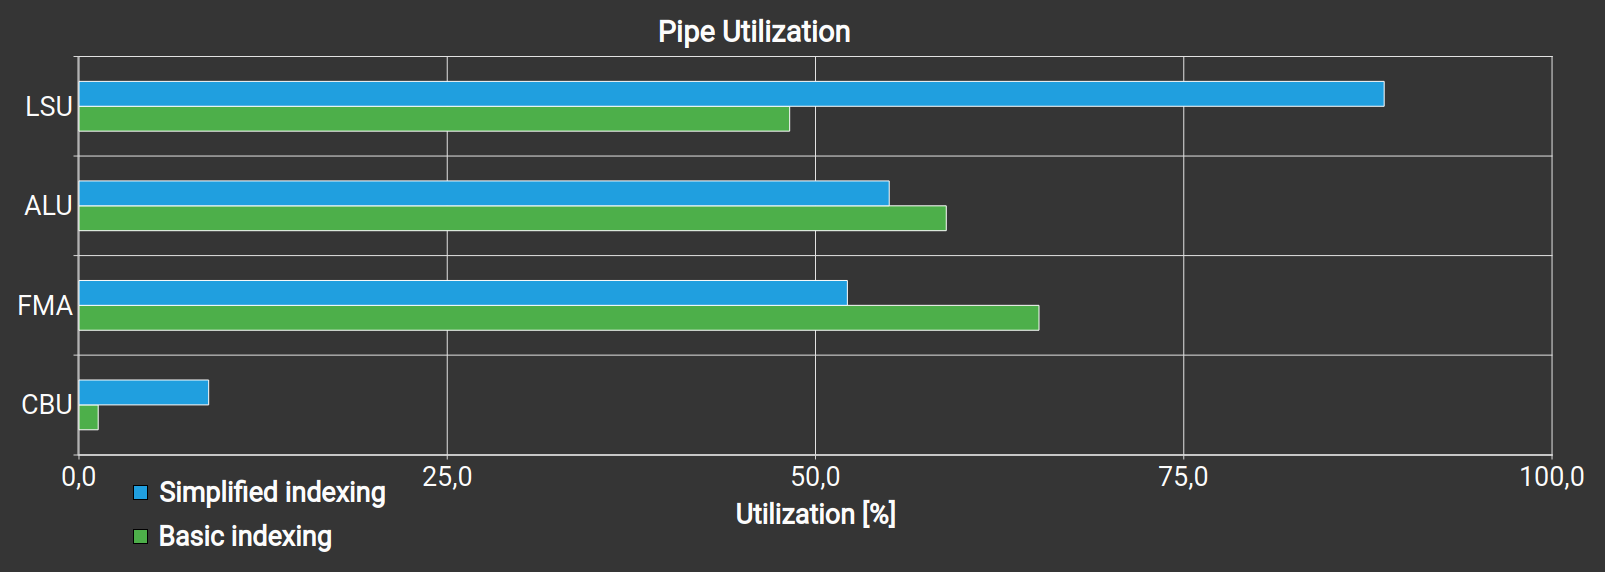
\includegraphics[width=\textwidth]{pipeline_utilization_simplified_indexing.png}
		\caption{Pipeline utilization.}
		\label{fig:pipeline_utilization_simplified_indexing}
	\end{subfigure}
	
	%\label{fig:warp_per_shift_indexing_comparison}
	\caption{Comparison of basic and simplified indexing.}
\end{figure}

The effects of different pipeline utilization can also be seen in Figure \ref{fig:warp_state_simplified_indexing}. Warps of basic indexing algorithm are mostly stalled due to not being selected, i.e. there are multiple eligible warps and only one of them can be issued. This indicates that there may be too many warps for the size of the GPU. As these benchmarks were run on a RTX 2060 mobile, which is a rather small GPU, this was to be expected. The other main reason of warp stall is \texttt{Stall Math Pipe Throttle}, which is caused by the high utilization of \textit{ALU} and \textit{FMA} pipelines. These pipelines are responsible for computing the indices and the actual results of cross-correlation, which represents the useful work done by the GPU.

Simple indexing warps on the other hand are more often stalled on the \texttt{Stall Wait}, which represents warps waiting for a fixed latency execution dependency, i.e. a data dependency between two instructions or an instruction dependency on predicate computation. We can also see noticeable increase in stalls due to access to global memory (\texttt{Stall Long Scoreboard} and \texttt{Stall LG Throttle}) together with stalls due to branching. This is consistent with the properties of simple indexing described above.

\begin{figure}[ht]
	\centering
	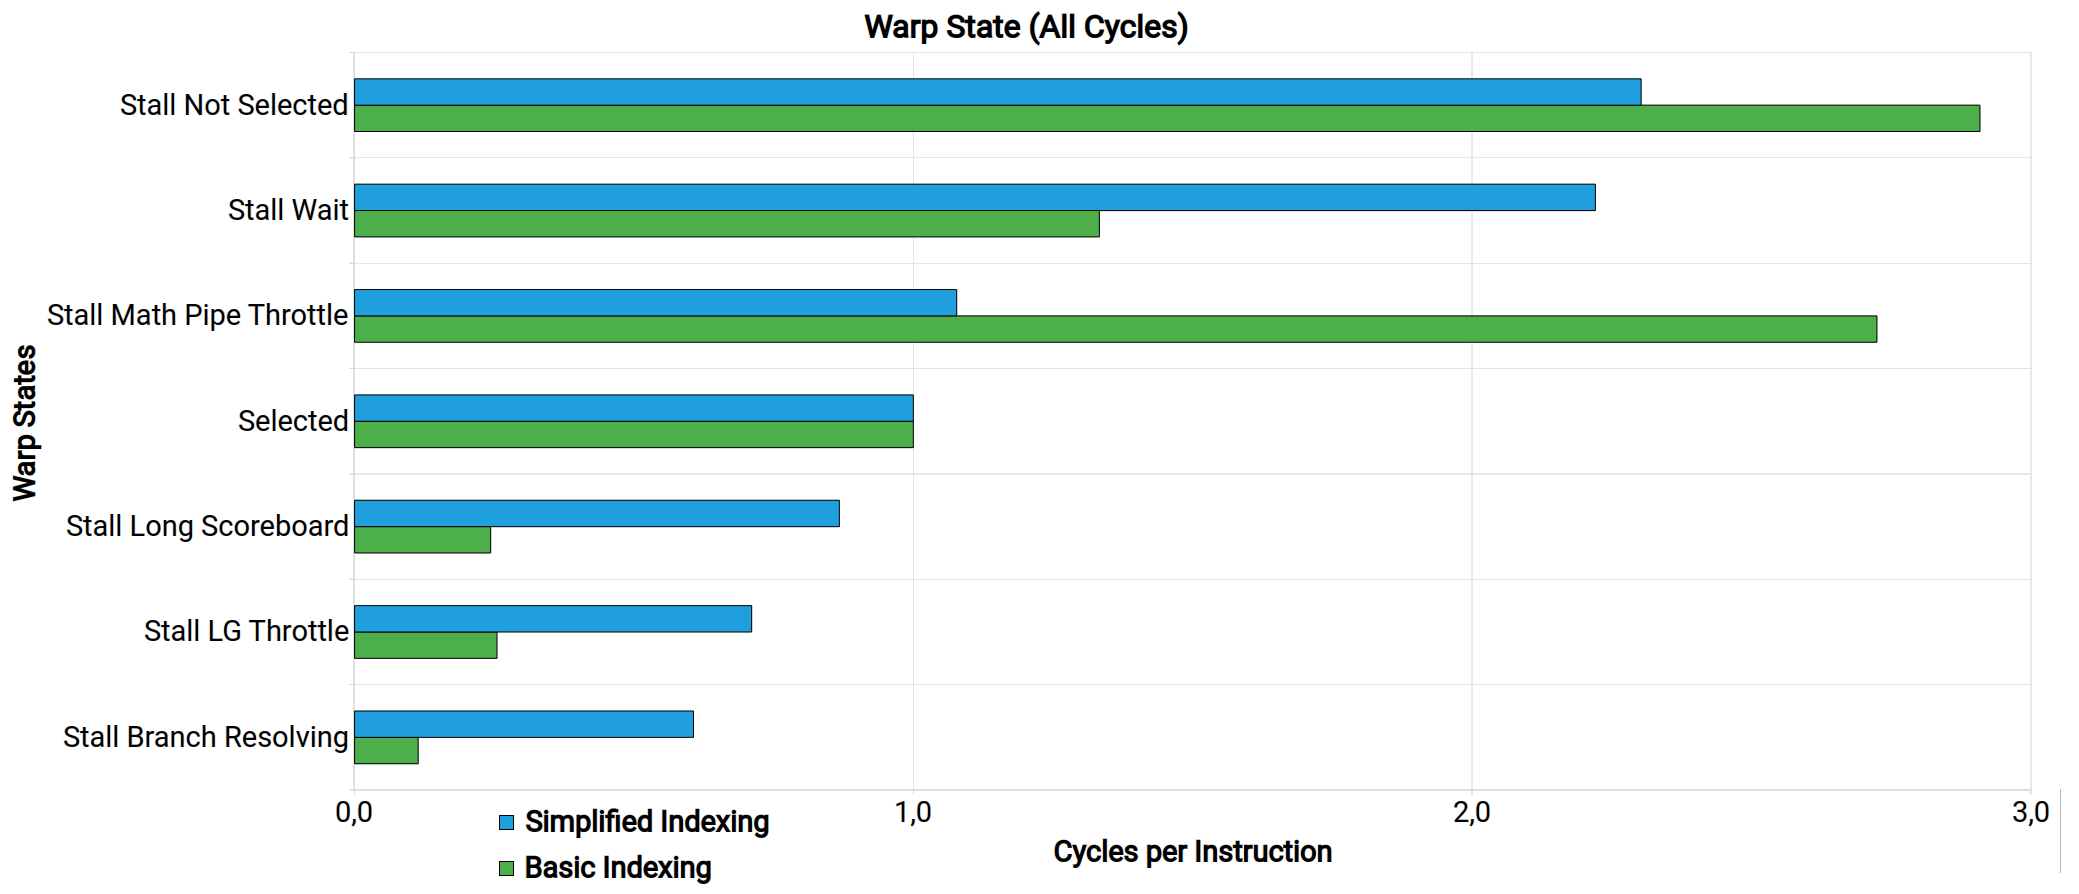
\includegraphics[width=0.8\textwidth]{warp_state_simplified_indexing.png}
	\caption{Comparison of warp stall reasons between the basic and simplified indexing.}
	\label{fig:warp_state_simplified_indexing}
\end{figure}

\subsection{Shared memory}
\label{sec:warp_per_shift_shared_mem}

% REFERENCE https://link.springer.com/content/pdf/10.1007/978-3-642-38718-0_38.pdf Access to shared memory to reduce accesses to global memory, block size, max blocks per SM etc.
This optimization of the base Warp per shift implementation is based on the work by \citet{paper:parameter_optimization}, who evaluate the impact of global memory access, occupancy and other parameters on execution time of a CUDA implementation of Levenshtein edit distance. Their implementation loads input data into shared memory to reduce the number of accesses to global memory, which is exactly what we want to achieve here.

We also take inspiration from the warp shuffle algorithm and its \textit{multirow} optimization. Instead of sharing input values by shuffling and broadcasting across threads of a warp, we load input values into shared memory and reuse them by all warps of the thread block.

Similarly to the warp shuffle algorithm, we utilize two alternating parts forming a ring buffer for data from the left input matrix and a single buffer for data from the right input matrix. Compared to the warp shuffle algorithm, the buffers are placed in the shared memory and are shared by all warps of each thread block. The data is not shuffled across threads as was done by warp shuffle, instead staying in place until overwritten by next load of the buffer, with each warp accessing the subset of the buffer it requires. The windows of the input data loaded into buffers are not moved along the rows of the input matrices, but along a group of columns from top to bottom, processing the whole columns group before moving onto the next column group, as shown in Figure \ref{fig:shared_mem_buffer_iterations}. This access pattern is based on the work of \citet{paper:krulis_3d_block}, who access the columns between overlapping patches in similar way.


With appropriately sized column groups, this enables us to maximize the throughput when loading data from global memory using coalesced loads. The appropriate size here is multiple of 32, i.e. warp size.  We call this the \textit{shared\_mem\_row\_size}, as it is also the size of each row of the shared memory buffers. The number of rows in each of the three shared memory buffers (two for data from the left matrix and one for data from the right matrix) is a run-time algorithm argument and stored in variable \textit{shared\_mem\_num\_rows}.
Another reason we choose column groups instead of row groups is because of the way we assign overlaps to warps of a thread block. To prevent bank conflicts when accessing shared memory, we assign consecutive overlaps from a single column of the output matrix to the warps of a single thread block. This is explained in more detail further in this section.


\begin{figure}[ht]
	\centering	
	\begin{subfigure}{\textwidth}
		\centering
		\def\svgwidth{0.7\textwidth}
		\fontsize{8}{10}\selectfont
		% Must be relative to current directory
		% as input ignores graphicspath, which is
		% only for includegraphics{}
		\input{./img/warp_per_shift-ThreadBlockOverlapCorrect.pdf_tex}
		\caption{Computation of a single column group showcasing different warp offsets and left bottom buffer preload offset.}
		\label{fig:shared_mem_buffer_iterations}
	\end{subfigure}
	\hfill
	\begin{subfigure}{\textwidth}
		\centering
		\def\svgwidth{0.7\textwidth}
		\fontsize{8}{10}\selectfont
		% Must be relative to current directory
		% as input ignores graphicspath, which is
		% only for includegraphics{}
		\input{./img/warp_per_shift-ThreadBlockOverlapsWrong.pdf_tex}
		\caption{Cross-iteration dependency when the bottom part of the left buffer is not loaded with an offset during the first load.}
		\label{fig:left_buffer_no_preload}
	\end{subfigure}
	
	%\label{fig:warp_per_shift_indexing_comparison}
	\caption{Processing of a column group by the Warp per shift algorithm with shared memory optimization.}
\end{figure}

As warp shuffle algorithm had warp submatrix, i.e. submatrix of each of the input matrices containing elements required by any of the threads of the given warp, this algorithm computes thread block submatrix containing elements of the input matrices required by overlaps assigned to any of the warps of the given thread block . This thread block submatrix is what we partition into column groups and what we iterate over and load into the shared memory buffers.

The implementation is again made up of three nested for loops, which can be found in the attachments of this thesis in the file \texttt{code/src/naive\_warp\_per\_shift\_shared\_mem.cu} as the \texttt{ccn\_warp\_per\_shift\_shared\_mem} kernel. The outer loop iterates over column groups while the middle loop iterates over rows of the column group in \textit{shared\_mem\_num\_rows} sized steps. These loops are shown in Listing \ref{lst:shared_memory_outer}. Threads of the whole thread block go through these two loops synchronously to allow cooperation when loading data to the shared memory buffers. 

When loading the bottom part of the left shared memory buffer in the outer loop, we need to limit which rows are loaded to the buffer and offset the loaded rows, as shown in Figure \ref{fig:shared_mem_buffer_iterations}. If we were to just load the full buffer as shown in Figure \ref{fig:left_buffer_no_preload}, we would encounter a situation where rows loaded in the second iteration of the middle loop into the right buffer overlap rows which were loaded during the first load of bottom left buffer, which at that point is already overwritten.  

\begin{lstlisting}[
style=cuda,
float,
caption=Outer and middle loop of the Warp per shift with shared memory optimizations,
label=lst:shared_memory_outer
]
T thread_sum = 0;
for (
	size_t column_group_start_x = block_matrix_start.x;
	column_group_start_x < block_matrix_end.x;
	column_group_start_x += shared_mem_row_size
) {
	// Bottom part of the left shared memory buffer
	left_bottom_s.load_submatrix(...);
	
	for (
		size_t right_buffer_start_row = block_matrix_start.y;
		right_buffer_start_row < block_matrix_end.y;
		right_buffer_start_row += shared_mem_num_rows
	) {
		left_top_s.load_submatrix(...);
		right_s.load_submatrix(...);
		
		__syncthreads();
		compute_from_shared_mem_buffers(left_bottom_s, right_s, ...);
		compute_from_shared_mem_buffers(left_top_s, right_s, ...);
		swap(left_bottom_s, left_top_s);
		__syncthreads();
	}
}
\end{lstlisting}


\begin{lstlisting}[
style=cuda,
float,
caption=Inner loop of the Warp per shift with shared memory optimizations accessing the shared memory buffers,
label=lst:shared_memory_inner
]
__device__ void compute_from_shared_mem_buffers(...) {
	// Offset in shared memory buffer
	int warp_right_start_offset = ...;
	int warp_right_end_offset = ...;
	// Offset between buffers
	int buffer_offset = ...;
	for (
		int right_idx = warp_right_start_offset + warp.thread_rank();
		right_idx < warp_right_end_offset;
		right_idx += warp.size()
	) {
		l = left_buffer[right_idx + buffer_offset];
		r = right_buffer[right_idx];
		thread_sum += l * r; 
	}
}
\end{lstlisting}

In each iteration, we compute the rows in the right buffer which overlap with rows in the given part of the left buffer in the overlap assigned to the current warp. The reason we have two parts of the left buffer is that different warps of a thread block will be computing different overlaps, as shown in the right column in Figure \ref{fig:shared_mem_buffer_iterations}. For $r$ rows loaded into right buffer, $w$ warps of a thread block will access $r + w - 1$ different rows from the left buffer based on the shift each warp is computing. The $w - 1$ rows will then be accessed by different warps in the following iteration as they compute shifts which overlap these rows of the left input matrix with rows of the right input matrix loaded into the right buffer in the following iteration. 



% Warps of a block compute consecutive shifts in Y axis

This innermost loop, shown in Listing \ref{lst:shared_memory_inner}, iterates over the rows from the two shared memory buffers which are overlapped in the overlap assigned to the current warp. Shared memory accesses in this loop are without bank conflicts thanks to way we assign overlaps between warps of a thread block. If we were to assign overlaps from a single row of the output matrix to warps of a thread block, as is done by the basic implementation of \textit{warp per shift} algorithm, we would encounter a problem illustrated in Figure \ref{fig:warp_per_shift_shared_mem_overlaps_in_x}. For the purposes of this example, we work with warps of 4 threads, shared memory with 4 banks and assume each input matrix fits into one shared memory buffer. The figure shows the left and right input matrix and how their elements map into banks of shared memory when loaded by the thread block. For simplicity, we have chosen a thread block whose thread block submatrix contains whole input matrices as one of the overlaps computed by the thread block is the overlap with shift $[0, 0]$. When warps of a given thread block are assigned overlaps along a row of the output matrix, the overlaps differ in the number of columns. This leads to an access pattern with different stride in each warp. The strides for warps 1 and 2 result in 2-way bank conflicts, the stride for warp 0 results in 4-way bank conflict. With 32 threads per warp, this type of access would cause up to 32-way bank conflict, which would severely limit the shared memory throughput.


Due to this, we choose to assign overlaps from a single column to warps of a thread block. This assignment leads to access illustrated in Figure \ref{fig:warp_per_shift_shared_mem_shifts}. This figure depicts two iterations of the innermost loop, with the same simplifications as the previous figure.  As the overlaps differ in the number of rows, not columns, the access to shared memory has different starting and ending offset, but between these the access is perfectly linear and coalesced, each thread accessing different bank. Left buffer is accessed independently of the right buffer, so sharing banks between these buffers does not lead to bank conflicts.

\begin{figure}[ht]
	
	\centering	
	\begin{subfigure}{0.31\textwidth}
		\centering
		\def\svgwidth{\textwidth}
		\fontsize{6}{8}\selectfont
		% Must be relative to current directory
		% as input ignores graphicspath, which is
		% only for includegraphics{}
		\input{./img/warp_per_shift-SharedMemAlongX.pdf_tex}
		\caption{Iteration 1 when job contains overlaps from a row of the output matrix.}
		\label{fig:warp_per_shift_shared_mem_overlaps_in_x}
	\end{subfigure}
	\hfill
	\begin{subfigure}{0.5\textwidth}
		\centering
		\def\svgwidth{\textwidth}
		\fontsize{6}{8}\selectfont
		% Must be relative to current directory
		% as input ignores graphicspath, which is
		% only for includegraphics{}
		\input{./img/warp_per_shift-SharedMemAlongY.pdf_tex}
		\caption{The first two iterations when job contains overlaps from a column of the output matrix.}
		\label{fig:warp_per_shift_shared_mem_shifts}
	\end{subfigure}
	
	%\label{fig:warp_per_shift_indexing_comparison}
	\caption{Input matrices with numbers designating their mapping to shared memory banks and how they are accessed by 4 different warps of a single thread block.}
	
	
\end{figure}






% 	Its basically very similar to multirow optimization, just with workers of warp size
% 	And because they are warp size, we can compute bounds for each and stop them whenever
%	we need without thread divergence
Even with the throughput of shared memory, the load from shared memory \textit{LDS} instructions become a bottleneck, as shown in Figure \ref{fig:warp_state_shared_mem}. The memory input/output stall is caused by the memory input/output queue being full. This queue handles special math instructions, dynamic branches and most importantly for us the shared memory access instructions. Even with this bottleneck, the reduction in number of global memory accesses allows the warp per shift algorithm with shared memory optimization to be usable even for larger inputs, as will be shown in Section \ref{sec:results_definition_based}.

\begin{figure}[ht]
	\centering
	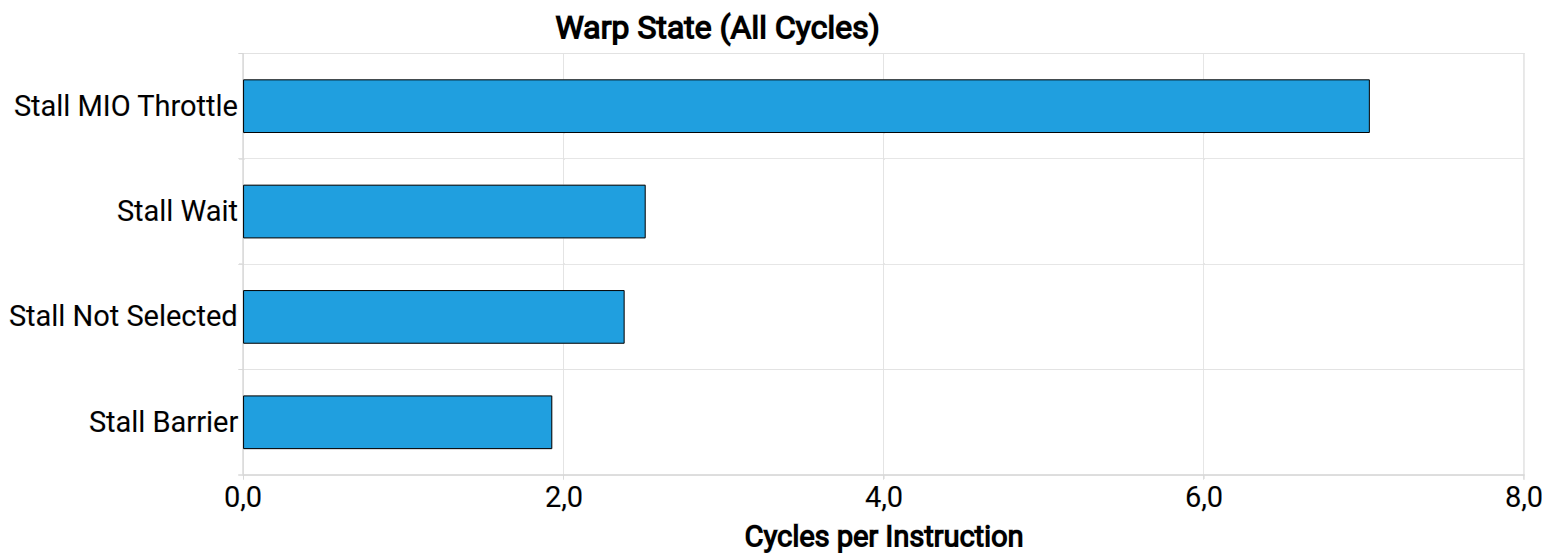
\includegraphics[width=0.8\textwidth]{warp_state_shared_mem.png}
	\caption{Memory input/output (MIO) stall caused by excessive shared memory access.}
	\label{fig:warp_state_shared_mem}
\end{figure}

\subsection{Shared memory with multiple right matrices}
\label{sec:warp_per_shift_shared_mem_multiright}

Similarly to the warp shuffle algorithm, we can increase the ratio of arithmetic instructions to shared memory loads by computing the same shift between a single left matrix and multiple right matrices. This improvement of the shared memory optimization is limited by the size of shared memory, as we need to fit multiple right shared memory buffers described in the previous section into shared memory at once. The code changes are very similar to the warp shuffle changes. We
again utilize the Local array optimization described in Appendix \ref{sec:local_array_optimization}, caching data in registers for reuse. We are computing overlaps with the same shift from different output matrices, as is done by the \textit{multimat\_right} optimization of the Warp shuffle family in Section \ref{sec:multimat_right}. Thanks to the same shift of all overlaps computed by given worker, any loop bounds computed hold for all the overlaps.

% TODO: Maybe code

The effects of this optimization are shown in Figure \ref{fig:shared_memory_multimat_right_profiling}. The profiling shows the difference between running the original shared memory optimization and running the shared memory optimization computing overlaps from multiple matrices at once. The profiling was done on $256 \times 256$ matrices, with one left input matrix and 16 right input matrices. The original shared memory optimization computes one overlap per warp, whereas the optimized version was run computing overlaps from eight matrices at once. The total number of shared memory load instructions (LDS) and memory access index computations using the integer multiply-add (IMAD) is significantly reduced, as the data from the left matrix once loaded into register is reused with data from eight right input matrices. Even with this reduction in the number of LDS instructions, the utilization of the \textit{LSU} pipeline is still a bottleneck, most likely due to the reduced throughput of shared memory in the Compute Capability 7.5 we use for profiling. The higher utilization of \textit{FMA} pipeline hints at better performance, which will be shown in Section \ref{sec:results_occupancy_improvements}.

\begin{figure}[ht]
	\centering	
	\begin{subfigure}{0.8\textwidth}
		\centering
		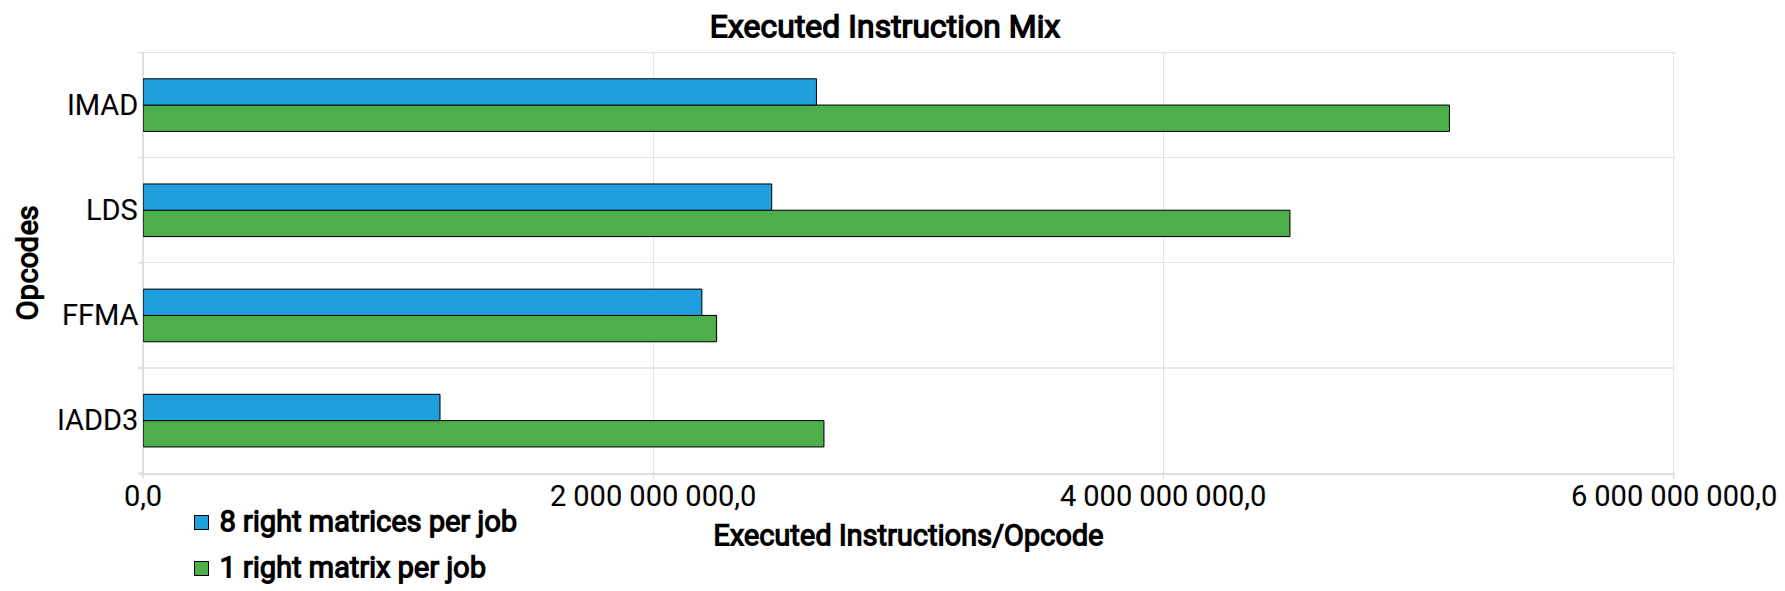
\includegraphics[width=\textwidth]{executed_instructions_shared_mem.png}
		\caption{Executed instructions.}
		%\label{fig:executed_instructions_shared_mem}
	\end{subfigure}
	\hfill
	\begin{subfigure}{0.8\textwidth}
		\centering
		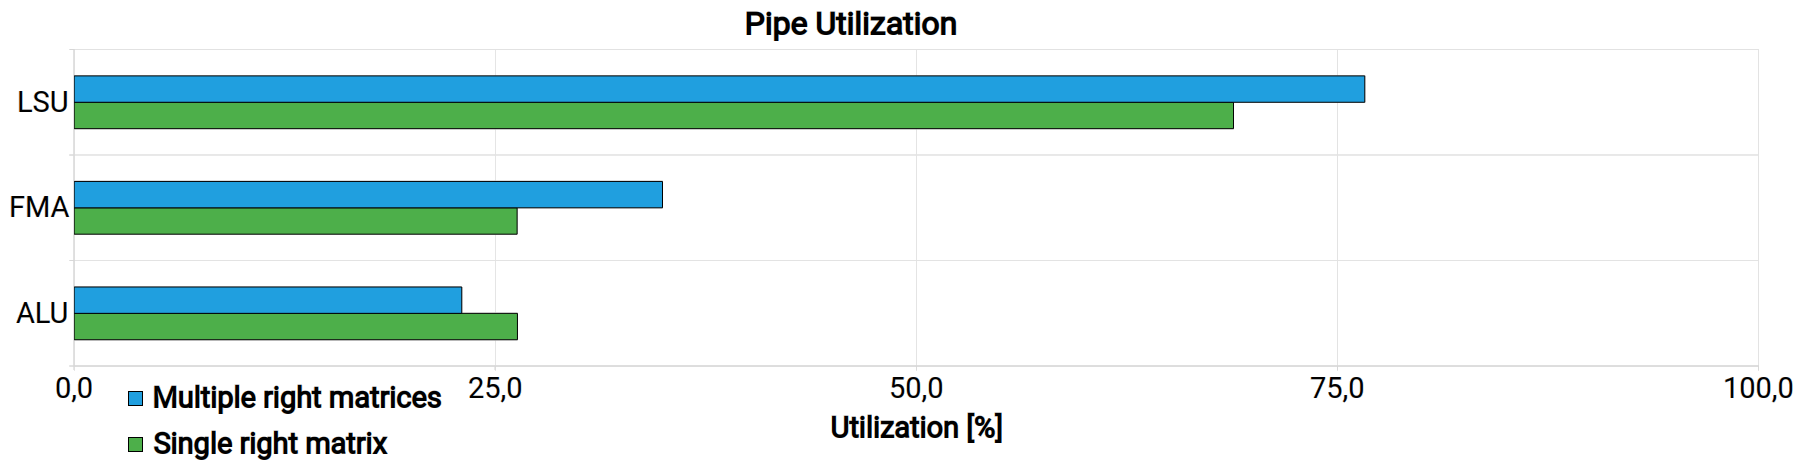
\includegraphics[width=\textwidth]{pipeline_utilization_shared_mem.png}
		\caption{Pipeline utilization.}
		%\label{fig:pipeline_utilization_shared_mem}
	\end{subfigure}
	
	\caption{Profiling of the effects of multiple right matrices on shared memory optimization.}
	\label{fig:shared_memory_multimat_right_profiling}
\end{figure}

\subsection{Shared memory with single column group per block}
\label{sec:column_group_per_worker}
As described in Section \ref{sec:warp_per_shift_shared_mem}, the thread block matrix is split into column groups. Each of these column groups can be processed independently, with the partial result added to the final result using \textit{atomicAdd} instruction as was done for the Work distribution optimization of the Warp shuffle algorithm family, introduced in Section \ref{sec:warp_shuffle_work_dist}. This improves the occupancy of the Warp per shift with shared memory optimization, possibly offsetting the reduced occupancy caused by overlaps from multiple overlaps grouped into each job introduced in Section \ref{sec:warp_per_shift_shared_mem_multiright}. The optimization further borrows from the rectangle work distribution, first computing the maximum number of column groups $m$ any overlap can be split into, and then starting $m$ workers for each overlap. As $m$ is the maximum number of column groups an overlap can be split into, most overlaps will be split into fewer column groups.  

This change should allow for additional parallelization as each column group is processed independently. The only change in terms of code of the CUDA kernel is the different computation of loop bounds and final store of the result using \textit{atomicAdd}, otherwise the code of the original implementation of the shared memory optimization can be reused without any changes. The effects of this change are evaluated in Section \ref{sec:results_occupancy_improvements}.

\subsection{Work distribution}
\label{sec:warp_per_shift_work_dist}

As described in Section \ref{sec:warp_shuffle_work_dist} with the warp shuffle algorithm, there are massive differences between work done by different workers in the basic algorithm. This optimization can only be applied to the base Warp per shift algorithm, as the use of Column groups by the shared memory optimization cannot be combined with Row groups used with work distribution. The implementation shares much of the code with the warp shuffle algorithm, only difference being the size of workers. We can choose from the \texttt{triangle} or \texttt{rectangle} distributions and set the maximum number of rows processed by a worker. The code of this optimization can be found in the attachments of this thesis in the file \texttt{code/src/naive\_warp\_per\_shift.cu} as the \texttt{ccn\_warp\_per\_shift\_work\_distribution} kernel.


This optimizations improves occupancy, further improving the main benefit of the Warp per shift family of algorithms. As described above, it also improves load balancing by reducing the differences between workloads of different workers. The disadvantage of this optimization is the reduced workload of each worker, which has to be balanced with the overhead of each worker such as scheduling, index calculations, atomic instructions to combine results from multiple workers etc. The optimization should provide improvements until the GPU is saturated. Additionally, without the use of shared memory described in Section \ref{sec:warp_per_shift_shared_mem}, the added strain onto global memory due to no data reuse between workers limits the performance of this optimization. 


\section{Further increasing worker size}
\label{sec:block_per_shift}
% REFERENCE file:///home/karel/skola/diplomka/crosscorr/papers/related_work/levenstein.pdf and their choice of size

% REFERENCE https://developer.nvidia.com/blog/faster-parallel-reductions-kepler/ for block reduction

Another possible way to further increase occupancy is to switch from warps as workers to whole thread blocks as workers. This can massively increase the number of threads started for given size of input, saturating the GPU even for smaller inputs. This optimization is again inspired by the work of \citet{paper:levenstein}, who assign stride, which is their unit of work, to be processed by a whole thread block. In our case, the implementation is rather simple. The thread block index directly maps to the position in the output matrix and consequently to the overlap computed by given thread block. This is why we call this the \textit{Block per shift} optimization. We then compute the bounds of the overlapping submatrix and iterate over the overlapping elements using block stride loop. We then utilize \texttt{reduce} function provided by Cooperative Groups API to sum results in each warp, which are then stored into shared memory and reduced again by warp 0 \citep{site:cuda_reduction}. The final result is then stored into the output matrix. 

This implementation should further improve occupancy, but at the cost of lower workload per thread, unbalanced workloads between workers and no data reuse. Based on our measurements presented in Section \ref{sec:results_occupancy_improvements}, this implementation does not improve run time over the base Warp per shift algorithm even for small input matrices. This is most likely caused by the simple warp per shift algorithm already saturating the GPU. Even for more powerful GPUs, the improved occupancy does not offset the problems listed above.

\subsection{Summary}

In this section, we have introduced the Warp per shift algorithm family and presented the following optimizations of this family:
\begin{itemize}
	\item simplified indexing (Section \ref{sec:simplified_indexing}),
	\item shared memory (Section \ref{sec:warp_per_shift_shared_mem}),
	\item shared memory with multiple right matrices (Section \ref{sec:warp_per_shift_shared_mem_multiright}),
	\item shared memory with column group per worker (Section \ref{sec:column_group_per_worker}),
	\item work distribution (Section \ref{sec:warp_per_shift_work_dist}).
\end{itemize}

The Warp per shift algorithm increases the worker size, utilizing whole warp to compute each job. The main goal of this family is to improve occupancy, saturating the GPU and utilizing its full throughput even for smaller inputs. The optimizations listed above then try to reduce overhead of the code caused by array indexing, introduce data reuse by loading data into shared memory and using them from multiple workers or further improve occupancy.

Using these optimizations, we have implemented the following versions of the Warp per shift algorithm:
\begin{itemize}
	\item base Warp per shift,
	\item Warp per shift with work distribution,
	\item Warp per shift with shared memory (combining all three optimizations).
\end{itemize}
	
We have also introduced one additional algorithm further optimizing for occupancy, the \textit{Block per shift} algorithm. 	Measurements and comparison of these algorithms and their implementations is presented in Section \ref{sec:results_occupancy_improvements}.





